%
%===================================================================================================
%
\documentclass[aspectratio=169]{beamer}
%
%===================================================================================================
%
% Theme and color scheme
\usetheme{Madrid}
\usecolortheme{default}
%
%===================================================================================================
%
% Packages
\usepackage[utf8]{inputenc}
\usepackage{amsmath}
\usepackage{amsfonts}
\usepackage{amssymb}
\usepackage{booktabs}
\usepackage{graphicx}
\usepackage{pgfpages}
\usepackage{framed}
\usepackage{xcolor}
\usepackage[most]{tcolorbox}
\usepackage{empheq}
\usepackage{bm}
\usepackage[absolute,overlay]{textpos}
\usepackage{minted}
\usepackage{hyperref}
%\usepackage{coffeestains}
%
%===================================================================================================
%
% Load tcolorbox listings support
\tcbuselibrary{listings}
%
%===================================================================================================
%
\usetikzlibrary{arrows.meta, positioning, calc, fit}
%
%===================================================================================================
%
% Custom colors for weights and biases

\definecolor{w1col}{RGB}{255,180,0}     % Yellow
\definecolor{w2col}{RGB}{180,90,30}     % Orange-brown
\definecolor{b1col}{RGB}{0,255,0}       % Green
\definecolor{accentred}{HTML}{E63946}
\definecolor{accentblue}{HTML}{457B9D}
\definecolor{codebg}{rgb}{0.97,0.97,0.97}
\definecolor{codeborder}{rgb}{0.8,0.8,0.8}
\definecolor{layer2red}{HTML}{FF0000}
\definecolor{layer1violet}{HTML}{800080}
\definecolor{updategreen}{HTML}{228B22}
%
%===================================================================================================
%
% Define custom code box

\newtcblisting{codebox}{
  listing only,
  colback=codebg,
  colframe=codeborder,
  arc=6pt,
  outer arc=6pt,
  boxrule=0.5pt,
  boxsep=4pt,
  left=4pt,
  right=4pt,
  top=4pt,
  bottom=4pt,
  listing options={
    language=Python,
    basicstyle=\ttfamily\small,
    keywordstyle=\color{blue}\bfseries,
    stringstyle=\color{orange},
    commentstyle=\color{gray},
    showstringspaces=false,
    breaklines=true,
    morekeywords={np}
  }
}

\newtcblisting{codebox2}{
  listing only,
  colback=codebg,
  colframe=codeborder,
  arc=6pt,
  outer arc=6pt,
  boxrule=0.5pt,
  boxsep=4pt,
  left=4pt,
  right=4pt,
  top=4pt,
  bottom=4pt,
  listing options={
    language=Python,
    basicstyle=\ttfamily\scriptsize,
    keywordstyle=\color{blue}\bfseries,
    stringstyle=\color{orange},
    commentstyle=\color{gray},
    showstringspaces=false,
    breaklines=true,
    morekeywords={np}
  }
}
%
%===================================================================================================
%
\DeclareUnicodeCharacter{FFFD}{ }
%
%===================================================================================================
%
\newcommand*{\itemimg}[1]{%
  \raisebox{-.3\baselineskip}{%
    \includegraphics[
      height=\baselineskip,
      width=\baselineskip,
      keepaspectratio,
    ]{#1}%
  }%
}

\newtcbox{\mymath}[1][]{%
    nobeforeafter, math upper, tcbox raise base,
    enhanced, colframe=blue!30!black,
    colback=blue!10, boxrule=1pt,
    #1}

\newcommand{\highlight}[1]{%
  \colorbox{yellow!100}{$\displaystyle#1$}}

\newcommand{\bx}{\bm{x}}
\newcommand{\bh}{\bm{h}}
\newcommand{\bw}{\bm{w}}
\newcommand{\bW}{\bm{W}}
\newcommand{\bb}{\bm{b}}
\newcommand{\R}{\mathbb{R}}

%
%===================================================================================================
%
% Title page information

\author{Giovanni Della Lunga\\{\footnotesize giovanni.dellalunga@unibo.it}}
\title{Chapter 1\\Introduction to Deep Learning}
\subtitle{} % (optional)
\setbeamercovered{transparent} 
\institute{Advanced Topics in Artificial Intelligence} 
\date{Bologna - March, 2026} 
%
%===================================================================================================
%
\begin{document}
%
%===================================================================================================
%
%\begin{frame}
%\includegraphics[width=\linewidth]{img/halloween-seminar-logo.PNG}
%\end{frame}
%
%===================================================================================================
%
\begin{frame}
\titlepage
\end{frame}
%
%===================================================================================================
%
\AtBeginSection[]
{
  %\begin{frame}<beamer>
  %\footnotesize	
  %\frametitle{Outline}
  %\begin{multicols}{2}
  %\tableofcontents[currentsection]
  %\end{multicols}	  
  %\normalsize
  %\end{frame}
  \begin{frame}
  \vfill
  \centering
  \begin{beamercolorbox}[sep=8pt,center,shadow=true,rounded=true]{title}  	\usebeamerfont{title}\insertsectionhead\par%
  \end{beamercolorbox}
  \vfill
  \end{frame}
}
\AtBeginSubsection{\frame{\subsectionpage}}
%
%===================================================================================================
%
% Table of contents
\begin{frame}{Contents}
    \setcounter{tocdepth}{1}
    \tableofcontents
\end{frame}
%__________________________________________________________________________
%
\section{Introduction}
%__________________________________________________________________________
%
\begin{frame}{About this Lesson}
In this lesson, we will cover the following topics:
\begin{itemize}
\item \textbf{Introduction to Deep Learning}. We will delve into the fundamental building block of deep learning, the neural network. We will cover the architecture of a neural network and its different components.
\item \textbf{The Feed Forward Architecture}. We will explore the simplest type of neural network, the feed-forward architecture, and learn how it can be used to solve a variety of problems. 
\item We begin by reviewing core building blocks such as logistic regression, the perceptron model, and gradient-based optimization. Then, we progressively extend these concepts to multi-layer neural networks
\item  Finally we will introduce the \textbf{modern deep learning toolkit}: activation functions (ReLU), optimizers (Adam), regularization techniques, and their application in financial models.
\end{itemize}
\end{frame}
%
%..................................................................
%
\begin{frame}{About this Lesson}

The focus of the lesson is both theoretical and practical: we aim to provide solid mathematical intuition, as well as hands-on coding experience through the implementation of key algorithms from scratch.
\\
\vspace {1cm}
By the end of the lesson, you should be able to:
\begin{itemize}
    \item Understand how deep learning models are trained and evaluated
    \item Implement basic architectures such as perceptrons and multilayer networks
    \item Analyze their performance on synthetic datasets
\end{itemize}
\end{frame}
%__________________________________________________________________________
%
\section{Artificial Neuron as Linear Classifier}
%__________________________________________________________________________
%
%__________________________________________________________________________
%
\subsection{Linear Separable Set}
%__________________________________________________________________________
%
\begin{frame}{Linear Separation}
\small
\textbf{Linearly Separable Data points}: Data points can be said to be linearly separable if a separating boundary/hyperplane can easily be drawn showing distinctively the different class groups. 
\begin{center}

\includegraphics[scale=0.35]{../05-pictures/ch-01-intro-to-deep-learning_pic_0.png}
\end{center}  
\end{frame}
%
%..................................................................
%
\begin{frame}{Linear Separation}
\begin{columns}
\begin{column}{.5\textwidth}
\textbf{Problem Definition}

\vspace{0.5cm}

Consider a simple 2D problem where each data point has two features ($x_1$ and $x_2$), and we want to classify them into two categories (let's call them \textbf{Class 1} and \textbf{Class 2}). 
\end{column}
\begin{column}{.5\textwidth}
\begin{center}

\includegraphics[scale=0.4]{../05-pictures/ch-01-intro-to-deep-learning_pic_1.png}
\end{center}  
\end{column}
\end{columns}
\end{frame}
%
%..................................................................
%
\begin{frame}{Linear Separation}
\begin{columns}
\begin{column}{.5\textwidth}
\textbf{Problem Definition}

\vspace{0.5cm}

A line can be drawn to separate the data points of \textbf{Class 1} from those of \textbf{Class 2}.\\
\vspace{0.3cm}
- \textbf{Class 1}: Points that lie on one side of the line (e.g., above the line)\\
\vspace{0.3cm}
- \textbf{Class 2}: Points that lie on the other side of the line (e.g., below the line).
\end{column}
\begin{column}{.5\textwidth}
\begin{center}

\includegraphics[scale=0.4]{../05-pictures/ch-01-intro-to-deep-learning_pic_1.png}
\end{center}
\end{column}  
\end{columns}
\end{frame}
%
%..................................................................
%
\begin{frame}{Linear Separation}
\textbf{Key Characteristics:}
\begin{itemize}
\item \textbf{2D Case}: In a two-dimensional dataset, the two classes can be separated by a straight line.
\item \textbf{Line Equation}: The separating line can be defined by the equation:

   $$
   w_1 x_1 + w_2 x_2 + b = 0
   $$

Where:\\
   - $x_1$ and $x_2$ are the features of the data points.\\
   - $w_1$ and $w_2$ are the weights (coefficients) that define the orientation of the line.\\
   - $b$ is the bias, which shifts the line vertically.

\end{itemize}
\end{frame}
%
%..................................................................
%
\begin{frame}{Geometrical Interpretation of W}{Linear Separation}
\begin{itemize}
\item The set of weights $(w_1, w_2)$ is nothing more than a vector $W$. \item But what exactly does $W$ represent? 
\item We can easily verify that the vector $\mathbf{w} = (w_1, w_2)$ is perpendicular to the line $w_1 x_1 + w_2 x_2 + b = 0$. 
\item To demonstrate this relationship we can use the following argument based on the properties of the dot product.
\end{itemize}
\end{frame}
%
%..................................................................
%
\begin{frame}{Geometrical Interpretation of W}{Linear Separation}
\begin{columns}[T] % align columns
\begin{column}{.5\textwidth}
\textbf{Step 1: Consider Two Points on the Line}
\vspace{0.5cm}
\begin{itemize}
\item Let $\mathbf{x} = (x_1, x_2)$ and $\mathbf{y} = (y_1, y_2)$ be any two distinct points on the line. 
\item Because both points lie on the line, they satisfy the equation:
$$
w_1 x_1 + w_2 x_2 + b = 0 
$$
$$
w_1 y_1 + w_2 y_2 + b = 0
$$
\end{itemize}
\end{column}%
\hfill%
\begin{column}{.5\textwidth}
	%\fbox{
		
\includegraphics[scale=.35]{../05-pictures/ch-01-intro-to-deep-learning_pic_2.png}
	%}
\end{column}%
\end{columns}
\end{frame}
%
%..................................................................
%
\begin{frame}{Geometrical Interpretation of W}{Linear Separation}
\begin{columns}[T] % align columns
\begin{column}{.5\textwidth}
\textbf{Step 2: Form a Tangent Vector to the Line}
\vspace{0.5cm}
\begin{itemize}
\item A vector that is tangent to the line can be obtained by taking the difference between the two points:

$$
\mathbf{v} = \mathbf{y} - \mathbf{x} = (y_1 - x_1, \, y_2 - x_2).
$$

\end{itemize}
\end{column}%
\hfill%
\begin{column}{.5\textwidth}
	%\fbox{
		
\includegraphics[scale=.35]{../05-pictures/ch-01-intro-to-deep-learning_pic_3.png}
	%}
\end{column}%
\end{columns}
\end{frame}
%
%..................................................................
%
\begin{frame}{Geometrical Interpretation of W}{Linear Separation}
\textbf{Step 3: Show That $\mathbf{w}$ is Perpendicular to $\mathbf{v}$}
\begin{itemize}
\item  To show that $\mathbf{w}$ is perpendicular to the tangent vector $\mathbf{v}$, we need to demonstrate that their dot product is zero:
$$
\mathbf{w} \cdot \mathbf{v} = w_1 (y_1 - x_1) + w_2 (y_2 - x_2).
$$
\begin{center}

\includegraphics[scale=0.3]{../05-pictures/ch-01-intro-to-deep-learning_pic_4.png}
\end{center}  
\end{itemize}
\end{frame}
%
%..................................................................
%
\begin{frame}{Geometrical Interpretation of W}{Linear Separation}
\textbf{Step 4: Use the Line Equations}
\begin{itemize}
\item Since both $\mathbf{x}$ and $\mathbf{y}$ lie on the line, we have:
$$
w_1 x_1 + w_2 x_2 + b = 0 \quad \Rightarrow \quad w_1 x_1 + w_2 x_2 = -b,
$$
$$
w_1 y_1 + w_2 y_2 + b = 0 \quad \Rightarrow \quad w_1 y_1 + w_2 y_2 = -b.
$$
\item Subtract the first equation from the second:
$$
(w_1 y_1 + w_2 y_2) - (w_1 x_1 + w_2 x_2) = -b - (-b) = 0.
$$
\item This simplifies to:
\begin{tcolorbox}
$$
w_1 (y_1 - x_1) + w_2 (y_2 - x_2) = 0 = \vec w \cdot (\vec y - \vec x) \quad \blacksquare
$$
\end{tcolorbox}
\end{itemize}
\end{frame}
%
%..................................................................
%
\begin{frame}{Describing Points Above or Below the Line}{Linear Separation}
Because the vector $ \mathbf{w} $ is perpendicular to the line, we can use it to “step off” the line in a controlled way. Specifically, consider any point of the form
$$
\mathbf{x} = \mathbf{x}_0 + \alpha\, \mathbf{u},
$$

where:\\
- $\mathbf{x}_0$ is a point on the line (so that $w_1 x_{1,0} + w_2 x_{2,0} + b = 0$),\\
- $\mathbf{u}$ is a unit vector in the direction of $ \mathbf{w} $, i.e.,

  $$
  \mathbf{u} = \frac{(w_1, w_2)}{\|\mathbf{w}\|},
  $$
\end{frame}
%
%..................................................................
%
\begin{frame}{Describing Points Above or Below the Line}{Linear Separation}
\begin{center}

\includegraphics[scale=0.45]{../05-pictures/ch-01-intro-to-deep-learning_pic_5.png}
\end{center}  
\end{frame}
%
%..................................................................
%
\begin{frame}{Describing Points Above or Below the Line}{Linear Separation}
\textbf{Evaluating the Linear Combination}
\vspace{0.5cm}
Let’s compute the value of
$$
f(\mathbf{x}) = w_1 x_1 + w_2 x_2 + b,
$$
for the point
$$
\mathbf{x} = \mathbf{x}_0 + \alpha\, \mathbf{u}.
$$
Substitute $\mathbf{x}$ into $f$:
$$
\begin{aligned}
f(\mathbf{x}) &= w_1 (x_{1,0} + \alpha u_1) + w_2 (x_{2,0} + \alpha u_2) + b \\
&= \bigl(w_1 x_{1,0} + w_2 x_{2,0} + b\bigr) + \alpha \bigl(w_1 u_1 + w_2 u_2\bigr).
\end{aligned}
$$
\end{frame}
%
%..................................................................
%
\begin{frame}{Describing Points Above or Below the Line}{Linear Separation}
Since $\mathbf{x}_0$ lies on the line, the first term is zero:
$$
w_1 x_{1,0} + w_2 x_{2,0} + b = 0.
$$
Now, consider the second term. Because $\mathbf{u}$ is the unit vector in the direction of $\mathbf{w}$:
$$
w_1 u_1 + w_2 u_2 = \mathbf{w} \cdot \mathbf{u} = \|\mathbf{w}\| \, \|\mathbf{u}\| \, \cos(0) = \|\mathbf{w}\| \cdot 1 \cdot 1 = \|\mathbf{w}\|.
$$
Thus, we have:
$$
f(\mathbf{x}) = \alpha \|\mathbf{w}\|.
$$
\end{frame}
%
%..................................................................
%
\begin{frame}{Describing Points Above or Below the Line}{Linear Separation}
\textbf{Interpreting the Result}

\vspace{.3cm}

\textbf{1. For Points Above the Line:}

\vspace{0.3cm}

   When $\alpha > 0$, we get
   $$
   f(\mathbf{x}) = \alpha \|\mathbf{w}\| > 0,
   $$
   because $\|\mathbf{w}\|$ is a positive quantity. Hence, all points that are a positive distance $\alpha$ from the line (in the direction of $ \mathbf{w} $) yield
   $$
   w_1 x_1 + w_2 x_2 + b > 0.
   $$
\end{frame}
%
%..................................................................
%
\begin{frame}{Describing Points Above or Below the Line}{Linear Separation}
\textbf{Interpreting the Result}

\vspace{0.3cm}

\textbf{2. For Points Below the Line:}

\vspace{0.3cm}

   When $\alpha < 0$, we obtain
   $$
   f(\mathbf{x}) = \alpha \|\mathbf{w}\| < 0,
   $$
   so all points that are a negative distance $\alpha$ from the line (opposite to the direction of $ \mathbf{w} $) yield
   $$
   w_1 x_1 + w_2 x_2 + b < 0.
   $$
\end{frame}
%
%..................................................................
%
\begin{frame}{}
\textbf{In the following section we will use three related but distinct objects:}
\begin{itemize}
  \item \textbf{Perceptron (Rosenblatt, 1958):} a linear classifier with a \emph{step} activation and a mistake-driven update rule.
  \item \textbf{Logistic Regression:} a \emph{probabilistic} model for binary labels with a Bernoulli likelihood, trained by maximizing likelihood (equivalently minimizing cross-entropy).
  \item \textbf{Sigmoid Neuron:} a differentiable computational unit that becomes a building block for neural networks.
\end{itemize}

\end{frame}
%__________________________________________________________________________
%
\subsection{Perceptron}
%__________________________________________________________________________
%
\begin{frame}{The Perceptron}
\begin{itemize}
\item The \textbf{Perceptron} is one of the simplest types of artificial neuron and is considered a foundational algorithm in machine learning and neural network theory. 
\item It was introduced by Frank Rosenblatt in 1958 and is primarily used for binary classification tasks, i.e., determining whether an input belongs to one of two classes.
\item A Perceptron works by classifying input vectors through a linear decision boundary, which \textbf{is adjusted during the training phase to minimize classification errors}.
\end{itemize}
\end{frame}
%
%..................................................................
%
\begin{frame}{The Perceptron}
\textbf{Model:}
\[
\hat{y} = \mathbb{I}\!\left(w^\top x + b \ge 0\right)\qquad \text{with } \hat{y}\in\{0,1\}.
\]
\textbf{Properties:}
\begin{itemize}
  \item Produces a \textbf{hard decision} (not a probability).
  \item Learns a \textbf{linear decision boundary}.
  \item Can solve \textbf{linearly separable} datasets; fails on XOR-like problems.
\end{itemize}
\end{frame}
%
%..................................................................
%
\begin{frame}{The Perceptron}
\centering

\includegraphics[scale=.375]{../05-pictures/ch-01-intro-to-deep-learning_pic_6.png} 
\end{frame}
%
%..................................................................
%
\begin{frame}{Perceptron Learning Rule}
Given a labeled example $(x_i, y_i)$ with $y_i\in\{0,1\}$:
\[
\hat{y}_i = \mathbb{I}(w^\top x_i + b \ge 0)
\]
\textbf{Update (only on mistakes):}
\[
w \leftarrow w + \eta (y_i - \hat{y}_i)x_i,
\qquad
b \leftarrow b + \eta (y_i - \hat{y}_i).
\]
\textbf{Important:}
\begin{itemize}
  \item This is \textbf{not} gradient descent on cross-entropy.
  \item The step activation is \textbf{not differentiable}, so standard backprop-style training does not apply.
\end{itemize}
\end{frame}
%
%..................................................................
%
\begin{frame}{The Perceptron}
\centering

\includegraphics[scale=.4]{../05-pictures/ch-01-intro-to-deep-learning_pic_7.png} 
\end{frame}
%
%..................................................................
%
\begin{frame}{What the Perceptron Is \emph{Not}}
\textbf{The perceptron is not:}
\begin{itemize}
  \item a probabilistic model ($\hat{y}$ is not a probability),
  \item trained by maximizing likelihood,
  \item trained by minimizing cross-entropy with gradient descent.
\end{itemize}
\medskip
\textbf{Then why do we still teach it?}
\begin{itemize}
  \item It is historically important and conceptually simple.
  \item It makes clear the limitation of linear separability.
  \item It motivates the transition to \textbf{differentiable} models.
\end{itemize}
\end{frame}
%__________________________________________________________________________
%
\subsection{Logistic Regression and Sigmoid Neuron}
%__________________________________________________________________________
%
\begin{frame}{Logistic Regression: A Probabilistic Model}
\textbf{Goal:} model the conditional probability of class $1$:
\[
P(y=1\mid x) = \sigma(w^\top x + b),
\qquad
\sigma(t)=\frac{1}{1+e^{-t}}.
\]
\textbf{Interpretation:}
\begin{itemize}
  \item Output is a \textbf{probability} in $(0,1)$.
  \item Labels are modeled as:
  \[
  y \mid x \sim \mathrm{Bernoulli}(a), \quad a=\sigma(w^\top x+b).
  \]
\end{itemize}
\end{frame}
%
%..................................................................
%
\begin{frame}{Likelihood and Cross-Entropy (Where the Loss Comes From)}
Given data $\{(x_i,y_i)\}_{i=1}^m$ with $y_i\in\{0,1\}$ and $a_i=\sigma(w^\top x_i+b)$:
\[
P(y_i\mid x_i; w,b) = a_i^{y_i}(1-a_i)^{1-y_i}.
\]
\textbf{Log-likelihood:}
\[
\log L(w,b) = \sum_{i=1}^m \left[y_i\log a_i + (1-y_i)\log(1-a_i)\right].
\]
\textbf{Training:} maximize $\log L$ \;\; $\Leftrightarrow$ \;\; minimize
\[
\mathcal{L}(w,b)= -\frac{1}{m}\sum_{i=1}^m \left[y_i\log a_i + (1-y_i)\log(1-a_i)\right]
\]
which is exactly the \textbf{binary cross-entropy}.
\end{frame}
%
%..................................................................
%
\begin{frame}{Why Logistic Regression Fits Deep Learning}
\textbf{Two crucial ingredients for modern neural networks:}
\begin{itemize}
  \item \textbf{Differentiability:} $\sigma(\cdot)$ is differentiable, so gradients exist.
  \item \textbf{A smooth objective:} cross-entropy is differentiable and works well with gradient-based optimization.
\end{itemize}
\medskip
This is the conceptual bridge from classical ML to deep learning:
\[
\text{Differentiable model} + \text{Differentiable loss} \Rightarrow \text{Gradient-based training}.
\]
\end{frame}
%
%..................................................................
%
\begin{frame}{Sigmoid Neuron}
\centering

\includegraphics[scale=.4]{../05-pictures/ch-01-intro-to-deep-learning_pic_8.png} 
\end{frame}
%
%..................................................................
%
\begin{frame}{Gradient Descent (For Logistic Regression)}
\textbf{Objective:} minimize $\mathcal{L}(w,b)$.
\[
w \leftarrow w - \eta \nabla_w \mathcal{L},
\qquad
b \leftarrow b - \eta \frac{\partial \mathcal{L}}{\partial b}.
\]
\textbf{Remark:}
\begin{itemize}
  \item This is standard for logistic regression because the model and loss are differentiable.
  \item This is \textbf{not} the historical perceptron learning rule.
\end{itemize}
\end{frame}
%
%..................................................................
%
\begin{frame}{Gradient Result (Logistic Regression)}
Let $A = \sigma(\mathbf{X}^T \cdot \mathbf{w} + \mathbf{b})$ (vector form), $y\in\mathbb{R}^{m\times 1}$.
Then:
\[
\nabla_w \mathcal{L} = \frac{1}{m}X^\top(A-y),
\qquad
\frac{\partial \mathcal{L}}{\partial b} = \frac{1}{m}\mathbf{1}^\top(A-y).
\]
\textbf{Interpretation:}
\begin{itemize}
  \item The term $(A-y)$ is the \textbf{prediction error} (in probability space).
  \item This pattern will reappear in backpropagation for multi-layer networks.
  \item In \textbf{Appendix A} you will find the complete derivation of this result.
\end{itemize}
\end{frame}
%__________________________________________________________________________
%
\subsection{Python Implementation}
%__________________________________________________________________________
%
\begin{frame}{Artificial Neuron Setup}
\begin{columns}[T] % align columns
\begin{column}{.48\textwidth}
Consider a simple artificial neuron for a 2D problem:
\begin{itemize}
    \item Inputs: $x_1, x_2$
    \item Weights: $w_1, w_2$
    \item Bias: $b$
    \item Activation function: sigmoid ($\sigma$)
\end{itemize}
\vspace{10pt}
The neuron's output is given by:
\[
\hat{y} = \sigma(z) = \sigma(w_1 x_1 + w_2 x_2 + b)
\]
\end{column}%
\hfill%
\begin{column}{.48\textwidth}
    %\fbox{
        
\includegraphics[width=\linewidth]{../05-pictures/ch-01-intro-to-deep-learning_pic_1.png}
    %}
\end{column}%
\end{columns}
\end{frame}
%
%..................................................................
%
\begin{frame}{Matrix Formulation}{Logistic Neuron Implementation}
\begin{itemize}
    \item Input matrix $X \in \mathbb{R}^{m \times n}$:
    \[
    X = \begin{bmatrix}
    x_1^{(1)} & x_2^{(1)} \\
    x_1^{(2)} & x_2^{(2)} \\
    \vdots & \vdots \\
    x_1^{(m)} & x_2^{(m)}
    \end{bmatrix}, \quad y = \begin{bmatrix}
    y^{(1)} \\
    y^{(2)} \\
    \vdots \\
    y^{(m)}
    \end{bmatrix} \in \mathbb{R}^{m \times 1}
    \]
    \item Weights vector: $w \in \mathbb{R}^{2 \times 1}$, bias $b \in \mathbb{R}$

$$   
W = \begin{bmatrix}
    w_{1} \\
    w_{2} 
    \end{bmatrix} \in \mathbb{R}^{2 \times 1}
$$
\end{itemize}
\end{frame}
%
%..................................................................
%
\begin{frame}{Matrix Formulation}{Logistic Neuron Implementation}
Define matrix $Z \in \mathbb{R}^{m \times 1}$ explicitly:
\vspace{0.5cm}
\begin{align*}
Z = X \cdot W + b &= \begin{bmatrix}
x_1^{(1)} & x_2^{(1)} \\
x_1^{(2)} & x_2^{(2)} \\
\vdots & \vdots \\
x_1^{(m)} & x_2^{(m)}
\end{bmatrix}
\cdot
\begin{bmatrix}
w_1 \\
w_2
\end{bmatrix}
+
\begin{bmatrix}
b \\
b \\
\vdots \\
b
\end{bmatrix} \\
&= \begin{bmatrix}
w_1 x_1^{(1)} + w_2 x_2^{(1)} + b \\
w_1 x_1^{(2)} + w_2 x_2^{(2)} + b \\
\vdots \\
w_1 x_1^{(m)} + w_2 x_2^{(m)} + b
\end{bmatrix}
\end{align*}
Dimensions: $(m,2)\cdot(2,1)+(m,1)=(m,1)$
\end{frame}
%
%..................................................................
%
\begin{frame}{Matrix Formulation}{Logistic Neuron Implementation}
Explicit vectorized gradient computation:
\[\frac{\partial \mathcal{L}}{\partial W} = 
\frac{1}{m}
\begin{bmatrix}
(a^{(1)} - y^{(1)})x_1^{(1)} + \dots + (a^{(m)} - y^{(m)})x_1^{(m)} \\
(a^{(1)} - y^{(1)})x_2^{(1)} + \dots + (a^{(m)} - y^{(m)})x_2^{(m)}
\end{bmatrix}
\]
can be compactly written as:
\[\frac{\partial \mathcal{L}}{\partial W} = \frac{1}{m}
\underbrace{
\textcolor{magenta}{
\begin{bmatrix}
x_1^{(1)} & x_1^{(2)} & \dots & x_1^{(m)} \\
x_2^{(1)} & x_2^{(2)} & \dots & x_2^{(m)}
\end{bmatrix}}}_{(2,m)}
\underbrace{
\left(
\textcolor{red}{
\begin{bmatrix}a^{(1)} \\ a^{(2)} \\ \vdots \\ a^{(m)}\end{bmatrix}}-
\textcolor{blue}{
\begin{bmatrix}y^{(1)} \\ y^{(2)} \\ \vdots \\ y^{(m)}\end{bmatrix}}
\right)}_{(m,1)}
\]
\[\mathbf{
\frac{\partial \mathcal{L}}{\partial W} = \frac{1}{m}
\textcolor{magenta}{\, X^T} \cdot \left( \textcolor{red} A - \textcolor{blue}y \right)
}
\]
\end{frame}
%
%..................................................................
%
\begin{frame}{Matrix Formulation}{Logistic Neuron Implementation}
We can easily generalize to $n$ features:
\vspace{0.5cm}
\begin{align*}
Z = X \cdot W + b &= \begin{bmatrix}
x_1^{(1)} & x_2^{(1)} & \dots   & x_n^{(1)} \\
x_1^{(2)} & x_2^{(2)} & \dots   & x_n^{(2)} \\
\vdots    & \vdots    & \ddots  & \vdots    \\
x_1^{(m)} & x_2^{(m)} & \dots   & x_n^{(m)}
\end{bmatrix}
\cdot
\begin{bmatrix}
w_1    \\
w_2    \\
\vdots \\
w_n
\end{bmatrix}
+
\begin{bmatrix}
b \\
b \\
\vdots \\
b
\end{bmatrix} \\
&= \begin{bmatrix}
w_1 x_1^{(1)} + w_2 x_2^{(1)} + \dots + w_n x_n^{(1)} + b \\
w_1 x_1^{(2)} + w_2 x_2^{(2)} + \dots + w_n x_n^{(2)} + b \\
\vdots \\
w_1 x_1^{(m)} + w_2 x_2^{(m)} + \dots + w_n x_n^{(m)} + b
\end{bmatrix}
\end{align*}
\end{frame}
%
%..................................................................
%
\begin{frame}[fragile]{Matrix Formulation}{Logistic Neuron Implementation}
\textbf{Gradient of Logistic Loss – Vectorized Form}
\vspace{.25cm}
\begin{align*}
\frac{\partial \mathcal{L}}{\partial \mathbf{W}} =
\begin{bmatrix}
\frac{\partial \mathcal{L}}{\partial w_1} \\
\frac{\partial \mathcal{L}}{\partial w_2} \\
\vdots \\
\frac{\partial \mathcal{L}}{\partial w_{n}}
\end{bmatrix}
&=
\begin{bmatrix}
\frac{1}{m} \sum_{i=1}^m (a^{(i)} - y^{(i)}) x_1^{(i)} \\
\frac{1}{m} \sum_{i=1}^m (a^{(i)} - y^{(i)}) x_2^{(i)} \\
\vdots \\
\frac{1}{m} \sum_{i=1}^m (a^{(i)} - y^{(i)}) x_{n}^{(i)}
\end{bmatrix} \\
&= \frac{1}{m}
\underbrace{
\begin{bmatrix}
x_1^{(1)} & x_1^{(2)} & \cdots & x_1^{(m)} \\
x_2^{(1)} & x_2^{(2)} & \cdots & x_2^{(m)} \\
\vdots    & \vdots    & \ddots & \vdots    \\
x_{n}^{(1)} & x_{n}^{(2)} & \cdots & x_{n}^{(m)}
\end{bmatrix}
}_{\textcolor{blue}{(n,\, m)}}
\cdot
\underbrace{
\left(
\begin{bmatrix}
a^{(1)} \\
a^{(2)} \\
\vdots \\
a^{(m)}
\end{bmatrix}
-
\begin{bmatrix}
y^{(1)} \\
y^{(2)} \\
\vdots \\
y^{(m)}
\end{bmatrix}
\right)
}_{\textcolor{red}{(m,\, 1)}}
\end{align*}
\end{frame}
%
%..................................................................
%
\begin{frame}{Python Code}
\begin{center}

\includegraphics[scale=.4]{../05-pictures/ch-01-intro-to-deep-learning_pic_9.png}
\end{center}
\end{frame}
%
%..................................................................
%
\begin{frame}[fragile]{Python Code - Initialization}{Logistic Neuron: Implementation}
    
    % --- Equation ---
    \vspace{0.2cm}
    \[
    X = 
    \begin{bmatrix}
    x_1^{(1)} & x_2^{(1)} & \dots & x_n^{(1)} \\
    x_1^{(2)} & x_2^{(2)} & \dots & x_n^{(2)} \\
    \vdots & \vdots & \ddots & \vdots \\
    x_1^{(m)} & x_2^{(m)} & \dots & x_n^{(m)}
    \end{bmatrix} 
    , \quad \quad
    \bm{W} = 
    \begin{bmatrix}
    w_1 \\ w_2 \\ \vdots \\ w_n
    \end{bmatrix} 
    \in \mathbb{R}^{n \times 1}, 
    \quad b \in \mathbb{R}
    \]

    % --- Code ---
    \vspace{0.5cm}
    \begin{codebox}
def initialisation(X):
    W = np.random.randn(X.shape[1], 1)
    b = np.random.randn(1)
    return (W, b)
    \end{codebox}

\end{frame}
%
%..................................................................
%
\begin{frame}[fragile]{Python Code - Model}{Logistic Neuron: Implementation}
    
    % --- Equation ---
    \vspace{0.2cm}
    \[
    \bm{Z} = X \cdot W + b 
    , \quad \quad
    \bm{A} = \frac{1}{1+e^{-Z}}
    \]

    % --- Code ---
    \vspace{0.5cm}
    \begin{codebox}
def model(X, W, b):
    Z = X.dot(W) + b
    A = 1 / (1 + np.exp(-Z))
    return A
    \end{codebox}

\end{frame}
%
%..................................................................
%
\begin{frame}[fragile]{Python Code - Loss Function}{Logistic Neuron: Implementation}
    
    % --- Equation ---
    \vspace{0.2cm}
    \[
    \mathcal{L}(\mathbf{w}, b) = -\frac{1}{n} \sum\limits_{i=1}^n \left[ y^{(i)} \log a^{(i)} + (1 - y^{(i)}) \log(1 - a^{(i)}) \right]
    \]

    % --- Code ---
    \vspace{0.5cm}
    \begin{codebox}
def log_loss(A, y):
    return 1 / len(y) * np.sum(-y * np.log(A) - (1 - y) * np.log(1 - A))
    \end{codebox}

\end{frame}
%
%..................................................................
%
\begin{frame}[fragile]{Python Code - Gradient and Update}    
    % --- Equation ---
    \vspace{0.2cm}
    \[
    W = W - \alpha \frac{\partial \cal{L}}{\partial W}, \quad \quad 
    b = b - \alpha \frac{\partial \cal{L}}{\partial b} 
    \]

    % --- Code ---
    \vspace{0.2cm}
    \begin{codebox}
def gradients(A, X, y):
    dW = 1 / len(y) * np.dot(X.T, A - y)
    db = 1 / len(y) * np.sum(A - y)
    return (dW, db)
    
def update(dW, db, W, b, learning_rate):
    W = W - learning_rate * dW
    b = b - learning_rate * db
    return (W, b)
    \end{codebox}

\end{frame}
%
%..................................................................
%
\begin{frame}[fragile]{Python Code - Predict}{Logistic Neuron: Implementation}
    
    % --- Equation ---
    \vspace{0.2cm}
    \[
    A = \sigma \left(X \cdot W + b\right)    
    \]

    % --- Code ---
    \vspace{0.5cm}
    \begin{codebox}
def predict(X, W, b):
    A = model(X, W, b)
    # print(A)
    return A >= 0.5
    \end{codebox}

\end{frame}
%
%..................................................................
%
\begin{frame}[fragile]{Python Code}{Logistic Neuron: Implementation}
    \begin{codebox2}
def artificial_neuron(X, y, 
                      learning_rate = 0.1, 
                      n_iter = 250):
    W, b = initialisation(X)
    Loss = []
    history = []
    for i in range(n_iter):
        A = model(X, W, b)
        Loss.append(log_loss(A, y))
        dW, db = gradients(A, X, y)
        W, b = update(dW, db, W, b, learning_rate)
        history.append([W, b, Loss, i])
    y_pred = predict(X, W, b)
    print("Accuracy Score: ", accuracy_score(y, y_pred))
    plt.plot(Loss)
    plt.show()
    return (W, b, history)
\end{codebox2}

\end{frame}
%
%..................................................................
%
\begin{frame}{Summary: What We Will Build Upon}
\textbf{Perceptron (historical):}
\begin{itemize}
  \item hard decision $\mathbb{I}(w^\top x+b\ge 0)$
  \item mistake-driven updates
\end{itemize}

\medskip
\textbf{Logistic regression (modern baseline for deep learning):}
\begin{itemize}
  \item probabilistic output $\sigma(w^\top x+b)$
  \item Bernoulli likelihood $\Rightarrow$ cross-entropy
  \item gradient descent optimization
\end{itemize}

\end{frame}
%__________________________________________________________________________
%
\subsection{Non Linear Separable Sets\\ \small{Limits of the Single Neuron}}
%__________________________________________________________________________
%
\begin{frame}{Motivation: Where We Left Off}

We showed that \alert{logistic regression} solves the optimization problem
with a differentiable model and a smooth loss:
$$
  P(y=1\mid \bx) \;=\; \sigma(\bw^{\!\top}\bx + b)
$$

\medskip
\textbf{But it is still a linear classifier.}

\medskip
Its decision boundary is always a hyperplane --- no matter how we
tune $\bw$ and $b$.

\bigskip
\begin{block}{The question}
What happens when the data \textbf{cannot} be separated by a hyperplane?
\end{block}

\end{frame}
%
%..................................................................
%
\begin{frame}{The XOR Problem}

\begin{columns}[T]
\begin{column}{0.52\textwidth}

\includegraphics[scale=.5]{../05-pictures/ch-01-intro-to-deep-learning_pic_10.png}
\end{column}
\begin{column}{0.45\textwidth}
\textbf{Problem definition.}

\medskip
Class assignment depends on a \emph{nonlinear} rule:
\[
  y = 1 \;\;\text{iff}\;\; x_1 x_2 > 0
\]
i.e.\ points in \textbf{Quadrants I and III} belong to
\textcolor{accentred}{Class~1}, the rest to
\textcolor{accentblue}{Class~0}.

\bigskip
This is the classic \alert{XOR-like} pattern:
the label depends on the \emph{product} (interaction)
of the two features, not on each feature alone.
\end{column}
\end{columns}

\end{frame}
%
%..................................................................
%
\begin{frame}{Why a Single Neuron Fails}

\begin{columns}[T]
\begin{column}{0.52\textwidth}

\includegraphics[scale=.5]{../05-pictures/ch-01-intro-to-deep-learning_pic_11.png}
\end{column}
\begin{column}{0.45\textwidth}
No matter which line we try:
\[
  w_1 x_1 + w_2 x_2 + b = 0
\]
it \textbf{always} misclassifies a substantial fraction
of the data.

\bigskip
\textbf{The problem is not optimization.}

A logistic neuron can find the best possible line
--- but no line is good enough.

\bigskip
\alert{The problem is the \textbf{representation}:}
the raw features $(x_1, x_2)$ do not expose the
structure needed for a linear decision.
\end{column}
\end{columns}

\end{frame}
%
%..................................................................
%
\begin{frame}{The Core Idea: Learn a New Coordinate System}

\begin{block}{Key insight (Goodfellow et al., Ch.~6)}
Instead of classifying in the \emph{original} space, transform the
input into a \textbf{new space} where the problem \emph{becomes}
linearly separable.
\end{block}

\vspace{0.2cm}
Introduce a \alert{hidden layer} $\bh(\bx)$ with two neurons:
\[
  h_j(\bx) \;=\; \sigma\!\bigl(\bw_j^{\!\top}\bx + b_j\bigr),
  \qquad j = 1, 2
\]

Then classify in the \emph{transformed} space:
\[
  \bx \;\;\xrightarrow{\;\;\bh(\bx)\;\;}\;\;
  (h_1, h_2) \;\;\xrightarrow{\;\text{linear}\;\;}\;\; \hat{y}
\]

\vspace{0.2cm}
\textbf{The hidden layer does not add complexity for its own sake.}\\
It \emph{builds a coordinate system} in which a hyperplane suffices.

\end{frame}
%
%..................................................................
%
\begin{frame}{What Each Hidden Neuron Computes}

\begin{center}

\includegraphics[scale=.5]{../05-pictures/ch-01-intro-to-deep-learning_pic_12.png}
\end{center}

{\small
Each neuron partitions the original space with its own
\emph{linear boundary} and then ``squashes'' the result
through $\sigma$.
Individually, neither $h_1$ nor $h_2$ separates the classes
--- but \textbf{together} they create a representation where
a linear classifier succeeds.
}

\end{frame}
%
%..................................................................
%
\begin{frame}{Tracking Points: From $(x_1, x_2)$ to $(h_1, h_2)$}

\vspace{-4pt}
\begin{center}

\includegraphics[scale=.4]{../05-pictures/ch-01-intro-to-deep-learning_pic_13.png}
\end{center}

\vspace{-6pt}
{\footnotesize
\begin{tabular}{lccccl}
\toprule
 & $(x_1, x_2)$ & Quadrant & $h_1$ & $h_2$ & New coords \\
\midrule
$P_1$ & $(+0.79,\;+0.56)$ & I\;\textcolor{accentred}{(cls\,1)}
      & $0.59$ & $1.00$ & $(0.59,\; 1.00)$ \\
$P_2$ & $(-0.83,\;-0.59)$ & III\;\textcolor{accentred}{(cls\,1)}
      & $0.00$ & $0.27$ & $(0.00,\; 0.27)$ \\
$P_3$ & $(-1.17,\;+2.31)$ & II\;\textcolor{accentblue}{(cls\,0)}
      & $0.39$ & $1.00$ & $(0.39,\; 1.00)$ \\
$P_4$ & $(+1.46,\;-0.21)$ & IV\;\textcolor{accentblue}{(cls\,0)}
      & $0.47$ & $1.00$ & $(0.47,\; 1.00)$ \\
\bottomrule
\end{tabular}
\hfill
\parbox[b]{0.38\linewidth}{\raggedright
\textbf{Recipe:} read $h_1$ from the left panel, $h_2$ from the center.
The pair $(h_1, h_2)$ is the new address in the right panel.
}
}

\end{frame}
%
%..................................................................
%
\begin{frame}{The Transformed Space Is Linearly Separable}

\begin{columns}[T]
\begin{column}{0.52\textwidth}

\includegraphics[scale=.55]{../05-pictures/ch-01-intro-to-deep-learning_pic_14.png}
\end{column}
\begin{column}{0.45\textwidth}
After the hidden layer, each point $\bx$ is mapped
to coordinates $(h_1, h_2) \in (0,1)^2$.

\bigskip
In this new space the two classes occupy
\textbf{separable clusters}.

\bigskip
A single linear boundary
\[
  w_1' h_1 + w_2' h_2 + b' = 0
\]
now suffices (black line).

\bigskip
\alert{This is exactly what the output neuron does:}
it is a logistic regression in $\bh$-space.
\end{column}
\end{columns}

\end{frame}
%
%..................................................................
%
\begin{frame}{Side by Side: Original $\to$ Transformed}

\begin{center}

\includegraphics[scale=.45]{../05-pictures/ch-01-intro-to-deep-learning_pic_15.png}
\end{center}

\vspace{-4pt}
{\small
\textbf{Left:} no linear boundary works.
\hfill
\textbf{Right:} after $\bh(\bx)$, a straight line is all we need.

\smallskip
The hidden layer has \emph{learned} the feature interaction
that we would have had to engineer by hand (e.g.\ $x_1 x_2$).
}

\end{frame}
%
%..................................................................
%
\begin{frame}{The Decision Boundary Back in the Original Space}

\begin{columns}[T]
\begin{column}{0.52\textwidth}

\includegraphics[scale=.55]{../05-pictures/ch-01-intro-to-deep-learning_pic_16.png}
\end{column}
\begin{column}{0.45\textwidth}
When we map the linear boundary from $\bh$-space
\textbf{back} to $(x_1, x_2)$-space, it becomes a
\alert{nonlinear curve}.

\bigskip
The network has effectively learned:
\begin{enumerate}
\item A nonlinear feature map $\bh(\bx)$
\item A linear classifier in that space
\end{enumerate}

\bigskip
\textbf{Together}, these two steps produce a
complex decision boundary --- while each step
alone is simple.

\bigskip
This is the fundamental architecture of
\emph{every} feedforward neural network.
\end{column}
\end{columns}

\end{frame}
%
%..................................................................
%
\begin{frame}{Learning a Representation: Resume}

Instead of learning $x \rightarrow y$ directly, we change the objective:
\[
x \rightarrow h(x) \rightarrow y
\]

We transform the input $h(x) = \sigma(W^{[1]}x + b^{[1]})$, then classify:
\[
P(y=1|x)=\sigma(w^T h(x)+b)
\]

\textbf{This is the core idea of Deep Learning:}
\begin{itemize}
  \item We are not fitting a curve --- we are building a \textbf{coordinate system where the problem becomes linear}
  \item The hidden layer replaces manual feature design
\end{itemize}

\medskip
Classical ML: $\text{feature engineering} \rightarrow \text{model}$

Deep Learning: $\text{model} \rightarrow \text{features} \rightarrow \text{prediction}$
\end{frame}
%__________________________________________________________________________
%
\section{Neural Networks}
%__________________________________________________________________________
%
\subsection{Architecture}
%__________________________________________________________________________
%
\begin{frame}{Nodes and Layers}{Architecture}

The first step is to add some node making a \textbf{layer}
\vspace{1cm}

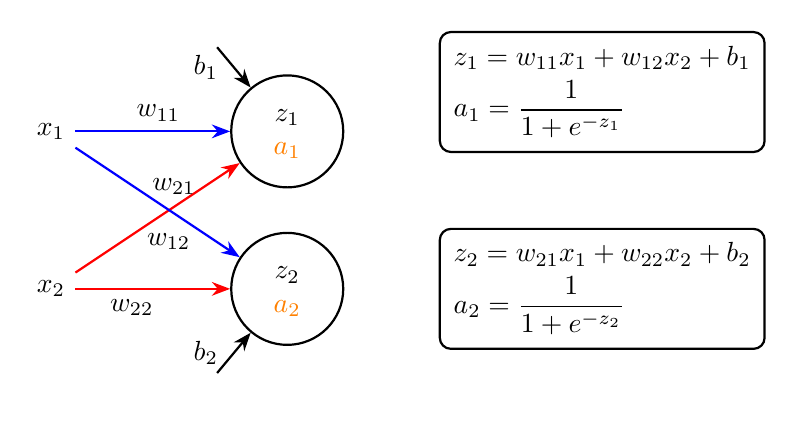
\begin{tikzpicture}[
    neuron/.style={circle, draw, minimum size=2.2em},  % Circle neurons
    input/.style={},                                   % Input style (no special style)
    ->, thick, >=Stealth                               % Arrows: thick with stealth tips
]

% --- INPUT NODES ---
\node[input] (x1) at (0,2) {$x_1$};
\node[input] (x2) at (0,0) {$x_2$};

% --- NEURONS ---
\node[neuron] (z1) at (3,2) {$\begin{array}{c} z_1 \\ \textcolor{orange}{a_1} \end{array}$};
\node[neuron] (z2) at (3,0) {$\begin{array}{c} z_2 \\ \textcolor{orange}{a_2} \end{array}$};

% --- CONNECTIONS WITH COLORED ARROWS AND LABEL ADJUSTMENTS ---
\draw[draw=blue] (x1) -- node[above, xshift=2pt] {$w_{11}$} (z1);             % x1 to z1 in blue
\draw[draw=red]  (x2) -- node[below, xshift=4pt, yshift=-2pt] {$w_{12}$} (z1); % x2 to z1 in red
\draw[draw=blue] (x1) -- node[above, pos=0.6, yshift=3pt] {$w_{21}$} (z2);    % x1 to z2 in blue
\draw[draw=red]  (x2) -- node[below, pos=0.4, xshift=-2pt] {$w_{22}$} (z2);   % x2 to z2 in red

% --- BIASES CONNECTED TO NEURONS (with label positioning) ---
\node[input] (b1) at (2,3.2) {};  % Bias for z1
\node[input] (b2) at (2,-1.2) {}; % Bias for z2

\draw[->] (b1) -- (z1) node[midway, left, xshift=-2pt] {$b_1$};  % Bias b1 arrow
\draw[->] (b2) -- (z2) node[midway, left, xshift=-2pt] {$b_2$};  % Bias b2 arrow

% --- EQUATIONS FOR z1 and a1 ---
\node[align=left, draw, rounded corners, inner sep=5pt] at (7,2.5) {
    $\displaystyle z_1 = w_{11}x_1 + w_{12}x_2 + b_1$ \\[0.3em]
    $\displaystyle a_1 = \frac{1}{1 + e^{-z_1}}$
};

% --- EQUATION FOR z2 ---
\node[align=left, draw, rounded corners, inner sep=5pt] at (7,0) {
    $\displaystyle z_2 = w_{21}x_1 + w_{22}x_2 + b_2$ \\[0.3em]
    $\displaystyle a_2 = \frac{1}{1 + e^{-z_2}}$
};

\end{tikzpicture}

\end{frame}
%
%..................................................................
%
\begin{frame}{Nodes and Layers}{Architecture}
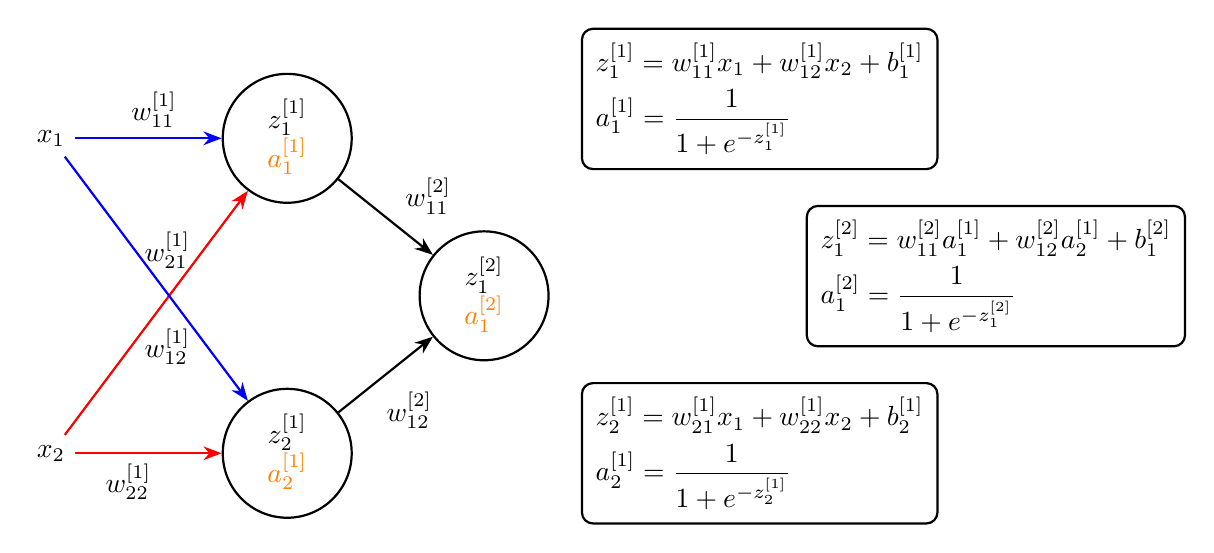
\begin{tikzpicture}[
    neuron/.style={circle, draw, minimum size=1em},
    input/.style={},
    ->, thick, >=Stealth
]

% --- INPUT NODES ---
\node[input] (x1) at (0,4) {$x_1$};
\node[input] (x2) at (0,0) {$x_2$};

% --- HIDDEN LAYER NEURONS ---
\node[neuron] (z1_1) at (3,4) {$\begin{array}{c} z_1^{[1]} \\ \textcolor{orange}{a_1^{[1]}} \end{array}$};
\node[neuron] (z2_1) at (3,0) {$\begin{array}{c} z_2^{[1]} \\ \textcolor{orange}{a_2^{[1]}} \end{array}$};

% --- OUTPUT NEURON ---
\node[neuron] (z1_2) at (5.5,2) {$\begin{array}{c} z_1^{[2]} \\ \textcolor{orange}{a_1^{[2]}}\end{array}$};
% centered between z1 and z2

% --- CONNECTIONS: INPUT TO HIDDEN ---
\draw[draw=blue] (x1) -- node[above, xshift=2pt] {$w_{11}^{[1]}$} (z1_1);
\draw[draw=red]  (x2) -- node[below, xshift=4pt, yshift=-2pt] {$w_{12}^{[1]}$} (z1_1);
\draw[draw=blue] (x1) -- node[above, xshift=4pt] {$w_{21}^{[1]}$} (z2_1);
\draw[draw=red]  (x2) -- node[below, pos=0.4, xshift=-2pt] {$w_{22}^{[1]}$} (z2_1);

% --- BIAS TO HIDDEN LAYER ---
%\node[input] (b1) at (2,3.2) {};
%\node[input] (b2) at (2,-1.2) {};
%\draw[->] (b1) -- (z1_1) node[midway, left, xshift=-2pt] {$b_1$};
%\draw[->] (b2) -- (z2_1) node[midway, left, xshift=-2pt] {$b_2$};

% --- CONNECTIONS: HIDDEN TO OUTPUT ---
\draw (z1_1) -- node[above right, pos=0.6] {$w_{11}^{[2]}$} (z1_2);
\draw (z2_1) -- node[below right, pos=0.4] {$w_{12}^{[2]}$} (z1_2);

% --- BIAS TO OUTPUT NODE ---
%\node[input] (b3) at (5,2.5) {};
%\draw[->] (b3) -- (z1_2) node[midway, left] {$b_3$};

% --- EQUATIONS FOR HIDDEN LAYER ---
\node[align=left, draw, rounded corners, inner sep=5pt] at (9,4.5) {
    $\displaystyle z_1^{[1]} = w_{11}^{[1]}x_1 + w_{12}^{[1]}x_2 + b_1^{[1]}$\\[0.3em]
    $\displaystyle a_1^{[1]} = \frac{1}{1 + e^{-z_1^{[1]}}}$
};

\node[align=left, draw, rounded corners, inner sep=5pt] at (9,0) {
    $\displaystyle z_2^{[1]} = w_{21}^{[1]}x_1 + w_{22}^{[1]}x_2 + b_2^{[1]}$\\[0.3em]
    $\displaystyle a_2^{[1]} = \frac{1}{1 + e^{-z_2^{[1]}}}$
};

% --- OUTPUT EQUATION ---
\node[align=left, draw, rounded corners, inner sep=5pt] at (12,2.25) {
    $\displaystyle z_1^{[2]} = w_{11}^{[2]}a_1^{[1]} + w_{12}^{[2]}a_2^{[1]} + b_1^{[2]}$\\[0.3em]
    $\displaystyle a_1^{[2]} = \frac{1}{1 + e^{-z_1^{[2]}}}$
};
\end{tikzpicture}
\end{frame}
%
%..................................................................
%
\begin{frame}{What the Network Is Actually Doing}

The network performs a sequence of computations:

\[
x \rightarrow z^{[1]} \rightarrow a^{[1]} \rightarrow z^{[2]} \rightarrow a^{[2]}
\]

Each neuron only does two things:

\[
\textbf{1) Linear combination}
\quad z = w^T x + b
\]

\[
\textbf{2) Nonlinear transformation}
\quad a = \sigma(z)
\]

A neural network is just the repeated application of these two steps.
\end{frame}
%
%..................................................................
%
\begin{frame}{Nodes and Layers}{Architecture}
As we know it's convenient to write in a more compact form the computation using the matrix notation:
\begin{equation}
\begin{pmatrix}
z_1 \\ z_2 \\ z_3 \\ z_4
\end{pmatrix} =
\begin{pmatrix}
w_{11} & w_{21} \\ w_{12} & w_{22} \\ w_{13} & w_{23} \\ w_{14} & w_{24}
\end{pmatrix} 
\cdot 
\begin{pmatrix}
x_1 \\ x_2 
\end{pmatrix}
+
\begin{pmatrix}
b_1 \\ b_2 \\ b_3 \\ b_4
\end{pmatrix} 
\Rightarrow Z^{[1]} = W^{[1]} \cdot X + B^{[1]} 
\end{equation}

$$ A^{[1]} = \sigma\left({Z^{[1]}}\right) $$
\end{frame}
%
%..................................................................
%
\begin{frame}{Nodes and Layers}{Architecture}
The result of the hidden layer is applied to the output node which will perform another linear operation with a different set of weights, $W^{[2]}$:
$$ Z^{[2]} = W^{[2]} \cdot A^{[1]} + B^{[2]} $$
and the final output will be the result of the application of the output node activation function to this value:
$$ \hat{y}  = A^{[2]}= \sigma\left({Z^{[2]}}\right)$$
\end{frame}
%__________________________________________________________________________
%
%\subsection{Backpropagation}
%__________________________________________________________________________
%
%__________________________________________________________________________
%
\subsection{The Network as a Mathematical Function}
%__________________________________________________________________________
%
\begin{frame}{What Are We Differentiating?}

Training a neural network means solving an optimization problem:

\[
\min_{\theta} L(\theta)
\]

But what exactly is the function \(L(\theta)\)?

Before computing derivatives, we must write the model as a single mathematical function.
\end{frame}
%
%..................................................................
%
\begin{frame}{The Network is a Function Composition}

The neural network is not a collection of equations.

It is a composition of functions:

\[
X
\;\xrightarrow{\,f_1\,}\;
Z^{[1]}
\;\xrightarrow{\,\sigma\,}\;
A^{[1]}
\;\xrightarrow{\,f_2\,}\;
Z^{[2]}
\;\xrightarrow{\,\sigma\,}\;
A^{[2]}
\]

Each block is a function applied to the output of the previous one.

Backpropagation will simply differentiate this composition.
\end{frame}
%
%..................................................................
%
\begin{frame}{Explicit Functional Form of the Network}

For a two-layer neural network:

\[
A^{[1]}(X) = \sigma(W^{[1]}X + b^{[1]})
\]

\[
A^{[2]}(X) = \sigma\!\left(W^{[2]}A^{[1]}(X) + b^{[2]}\right)
\]

Combining:

\[
A^{[2]}(X;\theta)
=
\sigma\!\left(
W^{[2]} \sigma(W^{[1]}X + b^{[1]}) + b^{[2]}
\right)
\]

This is a single function parameterized by \(\theta\).
\end{frame}
%
%..................................................................
%
\begin{frame}{The Loss Function}

We train the network using the cross-entropy loss:

\[
L(\theta)
=
-\frac{1}{m}
\sum_{i=1}^{m}
\left[
y_i \log A^{[2]}_i
+
(1-y_i)\log(1-A^{[2]}_i)
\right]
\]

The training problem is therefore:

\[
\min_{\theta} L(\theta)
\]

All backpropagation does is compute the gradient:

\[
\nabla_{\theta} L(\theta)
\]
\end{frame}
%__________________________________________________________________________
%
\subsection{Backpropagation}
%__________________________________________________________________________
%
\begin{frame}{Backpropagation for Logistic Regression}

Recall the result for a \textbf{single neuron}:
\vspace{0.1cm}
\begin{align*}
&Z = W \cdot X + b \quad \text{linear model}
\\
&A = \frac{1}{1 + e^{-Z}} \quad \text{activation function}
\\
&\mathcal{L} = -\frac{1}{m} \sum \left[ y \cdot \log(A) + (1 - y) \cdot \log(1 - A) \right] \quad \text{loss function}
\end{align*}
\textbf{Gradient equations}:
\begin{align*}
&\frac{\partial \mathcal{L}}{\partial W} = \frac{\partial \mathcal{L}}{\partial A} \cdot \frac{\partial A}{\partial Z} \cdot \frac{\partial Z}{\partial W}
\\&\\
&\frac{\partial \mathcal{L}}{\partial b} = \frac{\partial \mathcal{L}}{\partial A} \cdot \frac{\partial A}{\partial Z} \cdot \frac{\partial Z}{\partial b}
\end{align*}
\end{frame}
%
%..................................................................
%
\begin{frame}{Backpropagation for a 2-Layer Neural Network}
Now we have to calculate the gradient of the loss function with respect to each set of weights, one for each layer. 

\begin{align*}
A^{[2]} &= \sigma\left(Z^{[2]}\right) = \sigma \left( W^{[2]} \cdot A^{[1]} + B^{[2]} \right) \\
&= \sigma \left( W^{[2]} \cdot \sigma\left({Z^{[1]}}\right) + B^{[2]} \right) \\
&= \sigma \left[ W^{[2]} \cdot \sigma\left( W^{[1]} \cdot X + B^{[1]} \right) + B^{[2]} \right]
\end{align*}

\begin{tcolorbox}
As you can see $A^{[2]}$ depends on both $W^{[1]}$ and $W^{[2]}$. The specification of what a layer does to its input data is stored in the layer's weights. Remember once again that \textbf{learning means finding a set of values for the weights of all layers in a network, such that the network will correctly map example inputs to their associated targets} 
\end{tcolorbox}
\end{frame}
%
%..................................................................
%
\begin{frame}{Backpropagation for a 2-Layer Neural Network - 1}
\textbf{Gradient Computation for \textcolor{blue}{Layer 2}}
\begin{align*}
&Z^{[1]} = W^{[1]} \cdot X + b^{[1]}\\
&A^{[1]} = \frac{1}{1 + e^{-Z^{[1]}}}      \\
&Z^{[2]} = W^{[2]} \cdot A^{[1]} + b^{[2]} \\
&A^{[2]} = \frac{1}{1 + e^{-Z^{[2]}}} \\
&\textcolor{blue}{\mathcal{L} = -\frac{1}{m} \sum \left[ y \cdot \log(A^{[2]}) + (1 - y) \cdot \log(1 - A^{[2]}) \right]}
\end{align*}
\begin{align*}
&\frac{\partial \mathcal{L}}{\partial W^{[2]}} = \textcolor{blue}{\frac{\partial \mathcal{L}}{\partial A^{[2]}}} 
\\
&\frac{\partial \mathcal{L}}{\partial b^{[2]}} = \textcolor{blue}{\frac{\partial \mathcal{L}}{\partial A^{[2]}}} 
\end{align*}
\end{frame}
%
%..................................................................
%
\begin{frame}{Backpropagation for a 2-Layer Neural Network - 2}
\textbf{Gradient Computation for \textcolor{blue}{Layer 2}}
\begin{align*}
&Z^{[1]} = W^{[1]} \cdot X + b^{[1]}\\
&A^{[1]} = \frac{1}{1 + e^{-Z^{[1]}}}      \\
&Z^{[2]} = W^{[2]} \cdot A^{[1]} + b^{[2]} \\
&\textcolor{blue}{A^{[2]} = \frac{1}{1 + e^{-Z^{[2]}}}} \\
&\mathcal{L} = -\frac{1}{m} \sum \left[ y \cdot \log(A^{[2]}) + (1 - y) \cdot \log(1 - A^{[2]}) \right]
\end{align*}
\begin{align*}
&\frac{\partial \mathcal{L}}{\partial W^{[2]}} = \frac{\partial \mathcal{L}}{\partial A^{[2]}} \cdot \textcolor{blue}{\frac{\partial A^{[2]}}{\partial Z^{[2]}}} 
\\
&\frac{\partial \mathcal{L}}{\partial b^{[2]}} = \frac{\partial \mathcal{L}}{\partial A^{[2]}} \cdot \textcolor{blue}{\frac{\partial A^{[2]}}{\partial Z^{[2]}}} 
\end{align*}
\end{frame}
%
%..................................................................
%
\begin{frame}{Backpropagation for a 2-Layer Neural Network - 3}
\textbf{Gradient Computation for \textcolor{blue}{Layer 2}}
\begin{align*}
&Z^{[1]} = W^{[1]} \cdot X + b^{[1]}\\
&A^{[1]} = \frac{1}{1 + e^{-Z^{[1]}}}      \\
&\textcolor{blue}{Z^{[2]} = W^{[2]} \cdot A^{[1]} + b^{[2]}} \\
&A^{[2]} = \frac{1}{1 + e^{-Z^{[2]}}} \\
&\mathcal{L} = -\frac{1}{m} \sum \left[ y \cdot \log(A^{[2]}) + (1 - y) \cdot \log(1 - A^{[2]}) \right]
\end{align*}
\begin{align*}
&\frac{\partial \mathcal{L}}{\partial W^{[2]}} = \frac{\partial \mathcal{L}}{\partial A^{[2]}} \cdot \frac{\partial A^{[2]}}{\partial Z^{[2]}} \cdot \textcolor{blue}{\frac{\partial Z^{[2]}}{\partial W^{[2]}}}
\\
&\frac{\partial \mathcal{L}}{\partial b^{[2]}} = \frac{\partial \mathcal{L}}{\partial A^{[2]}} \cdot \frac{\partial A^{[2]}}{\partial Z^{[2]}} \cdot \textcolor{blue}{\frac{\partial Z^{[2]}}{\partial b^{[2]}}}
\end{align*}
\end{frame}
%
%..................................................................
%
\begin{frame}{Backpropagation for a 2-Layer Neural Network - 4}
\textbf{Gradient Computation for \textcolor{red}{Layer 1}}
\begin{align*}
&Z^{[1]} = W^{[1]} \cdot X + b^{[1]}\\
&A^{[1]} = \frac{1}{1 + e^{-Z^{[1]}}}      \\
&Z^{[2]} = W^{[2]} \cdot A^{[1]} + b^{[2]} \\
&A^{[2]} = \frac{1}{1 + e^{-Z^{[2]}}} \\
&\textcolor{blue}{\mathcal{L} = -\frac{1}{m} \sum \left[ y \cdot \log(A^{[2]}) + (1 - y) \cdot \log(1 - A^{[2]}) \right]}
\end{align*}
\begin{align*}
&\frac{\partial \mathcal{L}}{\partial W^{[1]}} = \textcolor{blue}{\frac{\partial \mathcal{L}}{\partial A^{[2]}}}
\\
&\frac{\partial \mathcal{L}}{\partial b^{[1]}} = \textcolor{blue}{\frac{\partial \mathcal{L}}{\partial A^{[2]}}}  
\end{align*}
\end{frame}
%
%..................................................................
%
\begin{frame}{Backpropagation for a 2-Layer Neural Network - 5}
\textbf{Gradient Computation for \textcolor{red}{Layer 1}}
\begin{align*}
&Z^{[1]} = W^{[1]} \cdot X + b^{[1]}\\
&A^{[1]} = \frac{1}{1 + e^{-Z^{[1]}}}      \\
&Z^{[2]} = W^{[2]} \cdot A^{[1]} + b^{[2]} \\
&\textcolor{blue}{A^{[2]} = \frac{1}{1 + e^{-Z^{[2]}}}} \\
&\mathcal{L} = -\frac{1}{m} \sum \left[ y \cdot \log(A^{[2]}) + (1 - y) \cdot \log(1 - A^{[2]}) \right]
\end{align*}
\begin{align*}
&\frac{\partial \mathcal{L}}{\partial W^{[1]}} = \frac{\partial \mathcal{L}}{\partial A^{[2]}} \cdot \textcolor{blue}{\frac{\partial A^{[2]}}{\partial Z^{[2]}}}
\\
&\frac{\partial \mathcal{L}}{\partial b^{[1]}} = \frac{\partial \mathcal{L}}{\partial A^{[2]}} \cdot \textcolor{blue}{\frac{\partial A^{[2]}}{\partial Z^{[2]}}}  
\end{align*}
\end{frame}
%
%..................................................................
%
\begin{frame}{Backpropagation for a 2-Layer Neural Network - 6}
\textbf{Gradient Computation for \textcolor{red}{Layer 1}}
\begin{align*}
&Z^{[1]} = W^{[1]} \cdot X + b^{[1]}\\
&A^{[1]} = \frac{1}{1 + e^{-Z^{[1]}}}      \\
&\textcolor{red}{Z^{[2]} = W^{[2]} \cdot A^{[1]} + b^{[2]}} \\
&A^{[2]} = \frac{1}{1 + e^{-Z^{[2]}}} \\
&\mathcal{L} = -\frac{1}{m} \sum \left[ y \cdot \log(A^{[2]}) + (1 - y) \cdot \log(1 - A^{[2]}) \right]
\end{align*}
\begin{align*}
&\frac{\partial \mathcal{L}}{\partial W^{[1]}} = \frac{\partial \mathcal{L}}{\partial A^{[2]}} \cdot \frac{\partial A^{[2]}}{\partial Z^{[2]}} \cdot \textcolor{red}{\frac{\partial Z^{[2]}}{\partial A^{[1]}}} 
\\
&\frac{\partial \mathcal{L}}{\partial b^{[1]}} = \frac{\partial \mathcal{L}}{\partial A^{[2]}} \cdot \frac{\partial A^{[2]}}{\partial Z^{[2]}} \cdot \textcolor{red}{\frac{\partial Z^{[2]}}{\partial A^{[1]}}}  
\end{align*}
\end{frame}
%
%..................................................................
%
\begin{frame}{Backpropagation for a 2-Layer Neural Network - 7}
\textbf{Gradient Computation for \textcolor{red}{Layer 1}}
\begin{align*}
&Z^{[1]} = W^{[1]} \cdot X + b^{[1]}\\
&\textcolor{red}{A^{[1]} = \frac{1}{1 + e^{-Z^{[1]}}}}      \\
&Z^{[2]} = W^{[2]} \cdot A^{[1]} + b^{[2]} \\
&A^{[2]} = \frac{1}{1 + e^{-Z^{[2]}}} \\
&\mathcal{L} = -\frac{1}{m} \sum \left[ y \cdot \log(A^{[2]}) + (1 - y) \cdot \log(1 - A^{[2]}) \right]
\end{align*}
\begin{align*}
&\frac{\partial \mathcal{L}}{\partial W^{[1]}} = \frac{\partial \mathcal{L}}{\partial A^{[2]}} \cdot \frac{\partial A^{[2]}}{\partial Z^{[2]}} \cdot \frac{\partial Z^{[2]}}{\partial A^{[1]}} \cdot \textcolor{red}{\frac{\partial A^{[1]}}{\partial Z^{[1]}}} 
\\
&\frac{\partial \mathcal{L}}{\partial b^{[1]}} = \frac{\partial \mathcal{L}}{\partial A^{[2]}} \cdot \frac{\partial A^{[2]}}{\partial Z^{[2]}} \cdot \frac{\partial Z^{[2]}}{\partial A^{[1]}} \cdot \textcolor{red}{\frac{\partial A^{[1]}}{\partial Z^{[1]}}} 
\end{align*}
\end{frame}
%
%..................................................................
%
\begin{frame}{Backpropagation for a 2-Layer Neural Network - 8}
\textbf{Gradient Computation for \textcolor{red}{Layer 1}}
\begin{align*}
&\textcolor{red}{Z^{[1]} = W^{[1]} \cdot X + b^{[1]}}\\
&A^{[1]} = \frac{1}{1 + e^{-Z^{[1]}}}      \\
&Z^{[2]} = W^{[2]} \cdot A^{[1]} + b^{[2]} \\
&A^{[2]} = \frac{1}{1 + e^{-Z^{[2]}}} \\
&\mathcal{L} = -\frac{1}{m} \sum \left[ y \cdot \log(A^{[2]}) + (1 - y) \cdot \log(1 - A^{[2]}) \right]
\end{align*}
\begin{align*}
&\frac{\partial \mathcal{L}}{\partial W^{[1]}} = \frac{\partial \mathcal{L}}{\partial A^{[2]}} \cdot \frac{\partial A^{[2]}}{\partial Z^{[2]}} \cdot \frac{\partial Z^{[2]}}{\partial A^{[1]}} \cdot \frac{\partial A^{[1]}}{\partial Z^{[1]}} \cdot \textcolor{red}{\frac{\partial Z^{[1]}}{\partial W^{[1]}}}
\\
&\frac{\partial \mathcal{L}}{\partial b^{[1]}} = \frac{\partial \mathcal{L}}{\partial A^{[2]}} \cdot \frac{\partial A^{[2]}}{\partial Z^{[2]}} \cdot \frac{\partial Z^{[2]}}{\partial A^{[1]}} \cdot \frac{\partial A^{[1]}}{\partial Z^{[1]}} \cdot \textcolor{red}{\frac{\partial Z^{[1]}}{\partial b^{[1]}}}
\end{align*}
\end{frame}
%
%..................................................................
%
\begin{frame}{Backpropagation for a 2-Layer Neural Network - 9}
\textbf{Let's simplify the gradient equations}
\begin{align*}
&\frac{\partial \mathcal{L}}{\partial W^{[2]}} = \frac{\partial \mathcal{L}}{\partial A^{[2]}} \cdot \frac{\partial A^{[2]}}{\partial Z^{[2]}} \cdot\frac{\partial Z^{[2]}}{\partial W^{[2]}}
\\
&\frac{\partial \mathcal{L}}{\partial b^{[2]}} = \frac{\partial \mathcal{L}}{\partial A^{[2]}} \cdot \frac{\partial A^{[2]}}{\partial Z^{[2]}} \cdot \frac{\partial Z^{[2]}}{\partial b^{[2]}}
\\
&\\
&\frac{\partial \mathcal{L}}{\partial W^{[1]}} = \frac{\partial \mathcal{L}}{\partial A^{[2]}} \cdot \frac{\partial A^{[2]}}{\partial Z^{[2]}} \cdot \frac{\partial Z^{[2]}}{\partial A^{[1]}} \cdot \frac{\partial A^{[1]}}{\partial Z^{[1]}} \cdot \frac{\partial Z^{[1]}}{\partial W^{[1]}}
\\
&\frac{\partial \mathcal{L}}{\partial b^{[1]}} = \frac{\partial \mathcal{L}}{\partial A^{[2]}} \cdot \frac{\partial A^{[2]}}{\partial Z^{[2]}} \cdot \frac{\partial Z^{[2]}}{\partial A^{[1]}} \cdot \frac{\partial A^{[1]}}{\partial Z^{[1]}} \cdot \frac{\partial Z^{[1]}}{\partial b^{[1]}}
\end{align*}
\end{frame}
%
%..................................................................
%
\begin{frame}{Backpropagation for a 2-Layer Neural Network - 10}
\textbf{Let's simplify the gradient equations}
\begin{align*}
&\frac{\partial \mathcal{L}}{\partial W^{[2]}} = \textcolor{blue}{\frac{\partial \mathcal{L}}{\partial A^{[2]}} \cdot \frac{\partial A^{[2]}}{\partial Z^{[2]}}} \cdot\frac{\partial Z^{[2]}}{\partial W^{[2]}}
\\
&\frac{\partial \mathcal{L}}{\partial b^{[2]}} = \textcolor{blue}{\frac{\partial \mathcal{L}}{\partial A^{[2]}} \cdot \frac{\partial A^{[2]}}{\partial Z^{[2]}}} \cdot \frac{\partial Z^{[2]}}{\partial b^{[2]}}
\\
&\\
&\frac{\partial \mathcal{L}}{\partial W^{[1]}} = \frac{\partial \mathcal{L}}{\partial A^{[2]}} \cdot \frac{\partial A^{[2]}}{\partial Z^{[2]}} \cdot \frac{\partial Z^{[2]}}{\partial A^{[1]}} \cdot \frac{\partial A^{[1]}}{\partial Z^{[1]}} \cdot \frac{\partial Z^{[1]}}{\partial W^{[1]}}
\\
&\frac{\partial \mathcal{L}}{\partial b^{[1]}} = \frac{\partial \mathcal{L}}{\partial A^{[2]}} \cdot \frac{\partial A^{[2]}}{\partial Z^{[2]}} \cdot \frac{\partial Z^{[2]}}{\partial A^{[1]}} \cdot \frac{\partial A^{[1]}}{\partial Z^{[1]}} \cdot \frac{\partial Z^{[1]}}{\partial b^{[1]}}
\end{align*}
\end{frame}
%
%..................................................................
%
\begin{frame}{Backpropagation for a 2-Layer Neural Network - 11}
\textbf{Let's simplify the gradient equations}
\begin{align*}
&dZ2 = \textcolor{blue}{\frac{\partial \mathcal{L}}{\partial A^{[2]}} \cdot \frac{\partial A^{[2]}}{\partial Z^{[2]}}} 
\\
&\frac{\partial \mathcal{L}}{\partial W^{[2]}} = \textcolor{blue}{dZ2} \cdot\frac{\partial Z^{[2]}}{\partial W^{[2]}}
\\
&\frac{\partial \mathcal{L}}{\partial b^{[2]}} = \textcolor{blue}{dZ2} \cdot \frac{\partial Z^{[2]}}{\partial b^{[2]}}
\\
&\\
&\frac{\partial \mathcal{L}}{\partial W^{[1]}} = \frac{\partial \mathcal{L}}{\partial A^{[2]}} \cdot \frac{\partial A^{[2]}}{\partial Z^{[2]}} \cdot \frac{\partial Z^{[2]}}{\partial A^{[1]}} \cdot \frac{\partial A^{[1]}}{\partial Z^{[1]}} \cdot \frac{\partial Z^{[1]}}{\partial W^{[1]}}
\\
&\frac{\partial \mathcal{L}}{\partial b^{[1]}} = \frac{\partial \mathcal{L}}{\partial A^{[2]}} \cdot \frac{\partial A^{[2]}}{\partial Z^{[2]}} \cdot \frac{\partial Z^{[2]}}{\partial A^{[1]}} \cdot \frac{\partial A^{[1]}}{\partial Z^{[1]}} \cdot \frac{\partial Z^{[1]}}{\partial b^{[1]}}
\end{align*}
\end{frame}
%
%..................................................................
%
\begin{frame}{Backpropagation for a 2-Layer Neural Network - 12}
\textbf{Let's simplify the gradient equations}
\begin{align*}
&dZ2 = \textcolor{blue}{\frac{\partial \mathcal{L}}{\partial A^{[2]}} \cdot \frac{\partial A^{[2]}}{\partial Z^{[2]}}} 
\\
&\frac{\partial \mathcal{L}}{\partial W^{[2]}} = \textcolor{blue}{dZ2} \cdot\frac{\partial Z^{[2]}}{\partial W^{[2]}}
\\
&\frac{\partial \mathcal{L}}{\partial b^{[2]}} = \textcolor{blue}{dZ2} \cdot \frac{\partial Z^{[2]}}{\partial b^{[2]}}
\\
&\\
&\frac{\partial \mathcal{L}}{\partial W^{[1]}} = \textcolor{red}{\frac{\partial \mathcal{L}}{\partial A^{[2]}} \cdot \frac{\partial A^{[2]}}{\partial Z^{[2]}} \cdot \frac{\partial Z^{[2]}}{\partial A^{[1]}} \cdot \frac{\partial A^{[1]}}{\partial Z^{[1]}}} \cdot \frac{\partial Z^{[1]}}{\partial W^{[1]}}
\\
&\frac{\partial \mathcal{L}}{\partial b^{[1]}} = \textcolor{red}{\frac{\partial \mathcal{L}}{\partial A^{[2]}} \cdot \frac{\partial A^{[2]}}{\partial Z^{[2]}} \cdot \frac{\partial Z^{[2]}}{\partial A^{[1]}} \cdot \frac{\partial A^{[1]}}{\partial Z^{[1]}}} \cdot \frac{\partial Z^{[1]}}{\partial b^{[1]}}
\end{align*}
\end{frame}
%
%..................................................................
%
\begin{frame}{Backpropagation for a 2-Layer Neural Network - 13}
\textbf{Let's simplify the gradient equations}
\begin{align*}
&dZ2 = \textcolor{blue}{\frac{\partial \mathcal{L}}{\partial A^{[2]}} \cdot \frac{\partial A^{[2]}}{\partial Z^{[2]}}} 
\\
&\frac{\partial \mathcal{L}}{\partial W^{[2]}} = \textcolor{blue}{dZ2} \cdot\frac{\partial Z^{[2]}}{\partial W^{[2]}}
\\
&\frac{\partial \mathcal{L}}{\partial b^{[2]}} = \textcolor{blue}{dZ2} \cdot \frac{\partial Z^{[2]}}{\partial b^{[2]}}
\\
&\\
&dZ1 = \textcolor{red}{\frac{\partial \mathcal{L}}{\partial A^{[2]}} \cdot \frac{\partial A^{[2]}}{\partial Z^{[2]}} \cdot \frac{\partial Z^{[2]}}{\partial A^{[1]}} \cdot \frac{\partial A^{[1]}}{\partial Z^{[1]}}}
\\
&\frac{\partial \mathcal{L}}{\partial W^{[1]}} = \textcolor{red}{dZ1} \cdot \frac{\partial Z^{[1]}}{\partial W^{[1]}}
\\
&\frac{\partial \mathcal{L}}{\partial b^{[1]}} = \textcolor{red}{dZ1} \cdot \frac{\partial Z^{[1]}}{\partial b^{[1]}}
\end{align*}
\end{frame}
%
%..................................................................
%
\begin{frame}{Backpropagation for a 2-Layer Neural Network - 14}
\textbf{Let's simplify the gradient equations}
\begin{align*}
&dZ2 = \textcolor{blue}{\frac{\partial \mathcal{L}}{\partial A^{[2]}} \cdot \frac{\partial A^{[2]}}{\partial Z^{[2]}}} 
\\
&\frac{\partial \mathcal{L}}{\partial W^{[2]}} = \textcolor{blue}{dZ2} \cdot\frac{\partial Z^{[2]}}{\partial W^{[2]}}
\\
&\frac{\partial \mathcal{L}}{\partial b^{[2]}} = \textcolor{blue}{dZ2} \cdot \frac{\partial Z^{[2]}}{\partial b^{[2]}}
\\
&\\
&dZ1 = \textcolor{blue}{dZ2} \cdot \textcolor{red}{\frac{\partial Z^{[2]}}{\partial A^{[1]}} \cdot \frac{\partial A^{[1]}}{\partial Z^{[1]}}}
\\
&\frac{\partial \mathcal{L}}{\partial W^{[1]}} = \textcolor{red}{dZ1} \cdot \frac{\partial Z^{[1]}}{\partial W^{[1]}}
\\
&\frac{\partial \mathcal{L}}{\partial b^{[1]}} = \textcolor{red}{dZ1} \cdot \frac{\partial Z^{[1]}}{\partial b^{[1]}}
\end{align*}
\end{frame}
%
%..................................................................
%
\begin{frame}{Backpropagation Through Two Layers}
\textbf{\textcolor{blue}{Computation of dZ2}}
\begin{itemize}
\item Given the loss function $L$ we defined above, we can easily compute the first partial derivative with respect to $\hat y$:

\begin{align*}
{\cal{L}} \left( y, A^{[2]}\right) &= -\left[ y\log{A^{[2]}} + \left( 1 - y \right)\log{\left(1 - A^{[2]}\right)}\right]\\ 
&\Downarrow \\
\frac{\partial \cal{L}}{\partial A^{[2]}} &= -\frac{y}{A^{[2]}} + \frac{1-y}{1-A^{[2]}} = \frac{\textcolor{red}{\mathbf{A^{[2]} - y}}}{A^{[2]}\cdot \left(1 - A^{[2]}\right)}
\end{align*}
\item Note that the numerator $\textcolor{red}{\mathbf{A^{[2]} - y}}$ is exactly the \textbf{prediction error} of the network! 
\end{itemize}
\end{frame}
%
%..................................................................
%
\begin{frame}{Backpropagation Through Two Layers}
\textbf{\textcolor{blue}{Computation of dZ2}}
\begin{align*}
\frac{\partial A^{[2]}}{\partial Z^{[2]}} &= \frac{\partial \sigma\left( Z^{[2]} \right)}{\partial Z^{[2]}} \\
&= \sigma\left(Z^{[2]}\right) \cdot \left[1 - \sigma\left(Z^{[2]}\right)\right]\\
&= A^{[2]} \left( 1 - A^{[2]} \right)
\end{align*}

\begin{align*}
dZ2 &= \textcolor{blue}{\frac{\partial \mathcal{L}}{\partial A^{[2]}} \cdot \frac{\partial A^{[2]}}{\partial Z^{[2]}}}  
\\
&=\frac{A^{[2]} - y}{A^{[2]}\cdot \left(1 - A^{[2]}\right)} \cdot A^{[2]} \left( 1 - A^{[2]} \right)
\\
&= A^{[2]} - y
\end{align*}
\end{frame}
%
%..................................................................
%
\begin{frame}{Backpropagation Through Two Layers}
\textbf{\textcolor{blue}{Computation of 2nd-Layer Gradients}}\\
Remembering that
\begin{align*}
&\textcolor{blue}{Z^{[2]} = W^{[2]} \cdot A^{[1]} + b^{[2]}} 
\end{align*}
We have 
\begin{align*}
\frac{\partial \mathcal{L}}{\partial W^{[2]}} &= dZ2 \cdot \textcolor{blue}{\frac{\partial Z^{[2]}}{\partial W^{[2]}}} = dZ2 \cdot A^{[1]} \\
&= \left( A^{[2]} - y \right) \cdot A^{[1]} 
\\&\\
\frac{\partial \mathcal{L}}{\partial b^{[2]}} &= dZ2 \cdot \textcolor{blue}{\frac{\partial Z^{[2]}}{\partial b^{[2]}}} = dZ2 \\
&= \left( A^{[2]} - y \right)
\end{align*}
\end{frame}
%
%..................................................................
%
\begin{frame}{Backpropagation Through Two Layers}
\textbf{\textcolor{blue}{Computation of dZ1}}
\begin{align*}
&dZ1 = dZ2 
\cdot 
\textcolor{red}{\frac{\partial Z^{[2]}}{\partial A^{[1]}}} 
\cdot 
\textcolor{blue}{\frac{\partial A^{[1]}}{\partial Z^{[1]}}}
\end{align*}
From
\begin{align*}
&Z^{[2]} = W^{[2]} \cdot A^{[1]} + b^{[2]} \\
&A^{[1]} = \sigma\left(Z^{[1]}\right)
\end{align*}
We have immediately
\begin{align*}
&\textcolor{red}{\frac{\partial Z^{[2]}}{\partial A^{[1]}}  = W^{[2]}} 
\\
&\textcolor{blue}{\frac{\partial A^{[1]}}{\partial Z^{[1]}} = 
\sigma\left( Z^{[1]} \right) \left[ 1-\sigma \left( Z^{[1]} \right) \right]
= A^{[1]} \left( 1 - A^{[1]} \right)}
\end{align*}
\begin{align*}
&\Rightarrow dZ1 = \left( A^{[2]} - y \right)
\cdot 
\textcolor{red}{W^{[2]}} 
\cdot
\textcolor{blue}{A^{[1]} \left( 1 - A^{[1]} \right)} 
\end{align*}
\end{frame}
%
%..................................................................
%
\begin{frame}{Backpropagation Through Two Layers}
\textbf{\textcolor{blue}{Computation of 1st-Layer Gradients}}\\

\begin{align*}
Z^{[1]} &= W^{[1]} \cdot X + b^{[1]} \\
&\\
\frac{\partial \mathcal{L}}{\partial W^{[1]}} &= 
\left( A^{[2]} - y \right)
\cdot 
W^{[2]} 
\cdot
A^{[1]} \left( 1 - A^{[1]} \right) 
\cdot 
\frac{\partial Z^{[1]}}{\partial W^{[1]}}
\\
&= \left( A^{[2]} - y \right)
\cdot 
W^{[2]} 
\cdot
A^{[1]} \left( 1 - A^{[1]} \right) 
\cdot 
X
\\&\\
\frac{\partial \mathcal{L}}{\partial b^{[1]}} &= 
\left( A^{[2]} - y \right)
\cdot 
W^{[2]} 
\cdot
A^{[1]} \left( 1 - A^{[1]} \right) 
\cdot 
\frac{\partial Z^{[1]}}{\partial b^{[1]}}
\\
&= \left( A^{[2]} - y \right)
\cdot 
W^{[2]} 
\cdot
A^{[1]} \left( 1 - A^{[1]} \right) 
\end{align*}
\end{frame}
%
%..................................................................
%
\begin{frame}{Backpropagation Through Two Layers}
Gradient equations for the 2-layer neural network (in red the 2nd layer, in violet the 1st):
\begin{align*}
&\textcolor{red}{dZ2 = \left( A^{[2]} - y \right)} 
\\
&\textcolor{red}{\frac{\partial \mathcal{L}}{\partial W^{[2]}} = dZ2 \cdot A^{[1]}} 
\\
&\textcolor{red}{\frac{\partial \mathcal{L}}{\partial b^{[2]}} = dZ2}
\\&\\
&\textcolor{violet}{dZ1 = \left( A^{[2]} - y \right)
\cdot 
W^{[2]} 
\cdot
A^{[1]} \left( 1 - A^{[1]} \right)} 
\\
&\textcolor{violet}{\frac{\partial \mathcal{L}}{\partial W^{[1]}} = dZ1 \cdot X}
\\
&\textcolor{violet}{\frac{\partial \mathcal{L}}{\partial b^{[1]}} = dZ1}
\end{align*}
\end{frame}
%
%..................................................................
%
\begin{frame}{The Computational Graph Behind Backpropagation}

All derivatives we are about to compute follow the same path:

\[
W^{[1]} \rightarrow Z^{[1]} \rightarrow A^{[1]} \rightarrow Z^{[2]} \rightarrow A^{[2]} \rightarrow L
\]

Backpropagation simply applies the chain rule along this graph:

\[
\frac{\partial L}{\partial W^{[1]}}
=
\frac{\partial L}{\partial A^{[2]}}
\frac{\partial A^{[2]}}{\partial Z^{[2]}}
\frac{\partial Z^{[2]}}{\partial A^{[1]}}
\frac{\partial A^{[1]}}{\partial Z^{[1]}}
\frac{\partial Z^{[1]}}{\partial W^{[1]}}
\]

We are not computing many formulas.

We are repeating the same rule along a path.
\end{frame}
%
%..................................................................
%
%
% --- CONDENSED: Chain Rule Applied Layer by Layer ---
%
\begin{frame}{Applying the Chain Rule: Layer 2}
Recall the full model:
\begin{align*}
&Z^{[1]} = W^{[1]} \cdot X + b^{[1]}, \quad A^{[1]} = \sigma(Z^{[1]})\\
&Z^{[2]} = W^{[2]} \cdot A^{[1]} + b^{[2]}, \quad A^{[2]} = \sigma(Z^{[2]})\\
&\mathcal{L} = -\frac{1}{m} \sum \left[ y \cdot \log(A^{[2]}) + (1 - y) \cdot \log(1 - A^{[2]}) \right]
\end{align*}

For the \textbf{output layer}, the chain rule gives:
\begin{align*}
&\frac{\partial \mathcal{L}}{\partial W^{[2]}} = \underbrace{\frac{\partial \mathcal{L}}{\partial A^{[2]}} \cdot \frac{\partial A^{[2]}}{\partial Z^{[2]}}}_{\textcolor{blue}{dZ2}} \cdot \frac{\partial Z^{[2]}}{\partial W^{[2]}}
\\[0.5em]
&\frac{\partial \mathcal{L}}{\partial b^{[2]}} = \textcolor{blue}{dZ2} \cdot \frac{\partial Z^{[2]}}{\partial b^{[2]}}
\end{align*}
\end{frame}
%
%..................................................................
%
\begin{frame}{Applying the Chain Rule: Layer 1}
For the \textbf{hidden layer}, the chain extends further back through the graph:
\begin{align*}
&\frac{\partial \mathcal{L}}{\partial W^{[1]}} = \underbrace{\textcolor{blue}{dZ2} \cdot \frac{\partial Z^{[2]}}{\partial A^{[1]}} \cdot \frac{\partial A^{[1]}}{\partial Z^{[1]}}}_{\textcolor{red}{dZ1}} \cdot \frac{\partial Z^{[1]}}{\partial W^{[1]}}
\\[0.5em]
&\frac{\partial \mathcal{L}}{\partial b^{[1]}} = \textcolor{red}{dZ1} \cdot \frac{\partial Z^{[1]}}{\partial b^{[1]}}
\end{align*}

\medskip
\textbf{Observe the recursive pattern:}
\begin{itemize}
\item Each layer computes a \textit{local error signal} $dZ^{[\ell]}$ from the layer above
\item The gradients for weights and biases follow the same form at every layer
\item This is the algorithm: \textbf{propagate $dZ$ backward, compute gradients locally}
\end{itemize}
\end{frame}
%
%..................................................................
%
\begin{frame}{Backpropagation Through Two Layers}
\framesubtitle{Complete Gradient Descent Update --- Putting It All Together}

\vspace{-0.15cm}

\begin{columns}[T]

% ---- LEFT: Gradient Formulas (Backpropagation) ----
\begin{column}{0.50\textwidth}

\small Step 1: \textbf{Compute Gradients (backward pass)}

{\small\color{layer2red}\textbf{Output Layer ($\ell = 2$):}}
{\small\color{layer2red}
\vspace{-0.15cm}
\begin{align*}
dZ^{[2]} &= A^{[2]} - y \\[-1pt]
dW^{[2]} &= \tfrac{1}{m}\, dZ^{[2]} \cdot {A^{[1]}}^{\!\top} \\[-1pt]
db^{[2]} &= \tfrac{1}{m} \textstyle\sum dZ^{[2]}
\end{align*}
}

{\small\color{layer1violet}\textbf{Hidden Layer ($\ell = 1$):}}
{\small\color{layer1violet}
\vspace{-0.15cm}
\begin{align*}
dZ^{[1]} &= {W^{[2]}}^{\!\top}\! \cdot dZ^{[2]} \odot A^{[1]}\!(1\!-\!A^{[1]}) \\[-1pt]
dW^{[1]} &= \tfrac{1}{m}\, dZ^{[1]} \cdot X^{\top} \\[-1pt]
db^{[1]} &= \tfrac{1}{m} \textstyle\sum dZ^{[1]}
\end{align*}
}

\end{column}

% ---- RIGHT: Update Rules (Gradient Descent) ----
\begin{column}{0.46\textwidth}

\small \textbf{Step 2: Update Parameters}

{\small\color{layer2red}\textbf{Output Layer ($\ell = 2$):}}
{\small
\begin{align*}
{\color{layer2red} \bm{W}^{[2]}} &\leftarrow W^{[2]} - {\color{updategreen}\eta} \cdot dW^{[2]} \\[3pt]
{\color{layer2red} \bm{b}^{[2]}} &\leftarrow b^{[2]} - {\color{updategreen}\eta} \cdot db^{[2]}
\end{align*}
}

{\small\color{layer1violet}\textbf{Hidden Layer ($\ell = 1$):}}
{\small
\begin{align*}
{\color{layer1violet} \bm{W}^{[1]}} &\leftarrow W^{[1]} - {\color{updategreen}\eta} \cdot dW^{[1]} \\[3pt]
{\color{layer1violet} \bm{b}^{[1]}} &\leftarrow b^{[1]} - {\color{updategreen}\eta} \cdot db^{[1]}
\end{align*}
}

\vspace{-0.15cm}

\colorbox{blue!8}{\parbox{0.92\linewidth}{\scriptsize
${\color{updategreen}\eta}$ = learning rate (hyperparameter)\\[1pt]
Repeat until convergence or early stopping.}}

\end{column}
\end{columns}

\end{frame}
%
%..................................................................
%
\begin{frame}{Backpropagation Through Two Layers}
\framesubtitle{Explicit Update Equations --- Fully Expanded Form}

\vspace{-0.1cm}

{\small Substituting the gradient expressions into $\theta \leftarrow \theta - \eta\, \nabla_\theta \mathcal{L}$\,:}

\vspace{0.15cm}

% ---- Layer 2 ----
{\small\color{layer2red}\textbf{Output Layer ($\ell = 2$):}}

\vspace{-0.05cm}

\begin{align}
{\color{layer2red}\bm{W}^{[2]}} &\leftarrow W^{[2]} \;-\; \frac{{\color{updategreen}\eta}}{m} \;\cdot\; \bigl(A^{[2]} - y\bigr) \;\cdot\; {A^{[1]}}^{\!\top} \label{eq:W2}\\[4pt]
{\color{layer2red}\bm{b}^{[2]}} &\leftarrow b^{[2]} \;-\; \frac{{\color{updategreen}\eta}}{m} \;\cdot\; \textstyle\sum \bigl(A^{[2]} - y\bigr) \label{eq:b2}
\end{align}

\vspace{0.05cm}

% ---- Layer 1 ----
{\small\color{layer1violet}\textbf{Hidden Layer ($\ell = 1$):}}

\vspace{-0.05cm}

\begin{align}
{\color{layer1violet}\bm{W}^{[1]}} &\leftarrow W^{[1]} \;-\; \frac{{\color{updategreen}\eta}}{m} \;\cdot\; \Bigl[\underbrace{{W^{[2]}}^{\!\top} \!\cdot\!\bigl(A^{[2]} - y\bigr)}_{\text{\scriptsize error backpropagated}} \;\odot\; \underbrace{A^{[1]}\!\bigl(1\!-\!A^{[1]}\bigr)}_{\text{\scriptsize local $\sigma'$}} \Bigr] \;\cdot\; X^{\top} \label{eq:W1}\\[4pt]
{\color{layer1violet}\bm{b}^{[1]}} &\leftarrow b^{[1]} \;-\; \frac{{\color{updategreen}\eta}}{m} \;\cdot\; \textstyle\sum \Bigl[{W^{[2]}}^{\!\top} \!\cdot\!\bigl(A^{[2]} - y\bigr) \;\odot\; A^{[1]}\!\bigl(1\!-\!A^{[1]}\bigr)\Bigr] \label{eq:b1}
\end{align}
\end{frame}
%
%..................................................................
%
\begin{frame}{Backpropagation Through Two Layers}
\framesubtitle{Explicit Update Equations --- Fully Expanded Form}

\colorbox{blue!8}{\parbox{0.96\linewidth}{\scriptsize
\textbf{Key:} The prediction error $\bigl(A^{[2]}\!-y\bigr)$ propagates through \emph{all} update equations. \;\; $\odot$ = element-wise (Hadamard) product. \;\; Eqs.~(\ref{eq:W1})--(\ref{eq:b1}) correspond to the Python functions \texttt{back\_propagation} + \texttt{update}.}}

\end{frame}
%__________________________________________________________________________
%
\subsection{Python Implementation}
%__________________________________________________________________________
%
\begin{frame}[fragile]
\frametitle{Weights Initialization}
\begin{itemize}
\item Our first neural network has 1 hidden layer and 2 layers in total (hidden layer + output layer), so there are 4 weight matrices to initialize ( $W^{[1]}$,$b^{[1]}$  and  $W^{[2]}$,$b^{[2]}$). 
\item n0: Number of neurons in the input layer; n1 : Number of neurons in the hidden layer; n2 : Number of neurons in the output layer.
\end{itemize}
\rule{\textwidth}{1pt}
\scriptsize
\begin{minted}{python}
def initialisation(n0, n1, n2):
    W1 = np.random.randn(n1, n0) 
    b1 = np.random.randn(n1, 1)
    W2 = np.random.randn(n2, n1) 
    b2 = np.random.randn(n2, 1)
    # Store all parameters in a dictionary for convenience
    parametres = {
        'W1': W1,  # Weights from input to hidden
        'b1': b1,  # Biases for hidden layer
        'W2': W2,  # Weights from hidden to output
        'b2': b2   # Biases for output layer
    }
    return parametres
\end{minted}
\rule{\textwidth}{1pt}
\end{frame}
%
%..................................................................
%
\begin{frame}[fragile]
\frametitle{Forward Propagation}
\scriptsize

\begin{align*}
A^{[2]} &= \sigma\left(Z^{[2]}\right) = \sigma \left( W^{[2]} \cdot A^{[1]} + B^{[2]} \right) = \sigma \left( W^{[2]} \cdot \sigma\left({Z^{[1]}}\right) + B^{[2]} \right) \\
&= \sigma \left[ W^{[2]} \cdot \sigma\left( W^{[1]} \cdot X + B^{[1]} \right) + B^{[2]} \right]
\end{align*}

\rule{\textwidth}{1pt}
\begin{minted}{python}

def forward_propagation(X, parametres):
    W1 = parametres['W1']  # Weights from input to hidden layer
    b1 = parametres['b1']  # Biases for hidden layer
    W2 = parametres['W2']  # Weights from hidden to output layer
    b2 = parametres['b2']  # Biases for output layer
    Z1 = W1.dot(X) + b1
    A1 = 1 / (1 + np.exp(-Z1))
    Z2 = W2.dot(A1) + b2
    A2 = 1 / (1 + np.exp(-Z2))
    activations = {
        'A1': A1,  # Activation from hidden layer
        'A2': A2   # Final prediction (output layer)
    }
    return activations
\end{minted}
\rule{\textwidth}{1pt}
\end{frame}
%
%..................................................................
%
\begin{frame}[fragile]
\frametitle{Backpropagation}
\rule{\textwidth}{1pt}
\scriptsize
\begin{minted}{python}

def back_propagation(X, Y, activations, parametres):
    A1 = activations['A1']  # Hidden layer activation
    A2 = activations['A2']  # Output layer activation (predicted probabilities)
    W2 = parametres['W2']  # Weights from hidden to output layer
    m = Y.shape[1]
    # -------- Backpropagation for Output Layer --------
    dz2 = A2 - Y  
    dW2 = (1 / m) * dz2.dot(A1.T)  
    db2 = (1 / m) * np.sum(dz2, axis=1, keepdims=True)  
    # -------- Backpropagation for Hidden Layer --------
    dz1 = W2.T.dot(dz2) * A1 * (1 - A1)  
    dW1 = (1 / m) * dz1.dot(X.T)  
    db1 = (1 / m) * np.sum(dz1, axis=1, keepdims=True)  
    gradients = {
        'dW1': dW1,
        'db1': db1,
        'dW2': dW2,
        'db2': db2
    }
    return gradients
\end{minted}
\rule{\textwidth}{1pt}
\end{frame}
%
%..................................................................
%
\begin{frame}[fragile]
\frametitle{Weights Update}
\rule{\textwidth}{1pt}
\scriptsize
\begin{minted}{python}

def update(gradients, parametres, learning_rate):
    W1 = parametres['W1']
    b1 = parametres['b1']
    W2 = parametres['W2']
    b2 = parametres['b2']
    dW1 = gradients['dW1']
    db1 = gradients['db1']
    dW2 = gradients['dW2']
    db2 = gradients['db2']
    W1 = W1 - learning_rate * dW1  # Update weights of layer 1
    b1 = b1 - learning_rate * db1  # Update biases of layer 1
    W2 = W2 - learning_rate * dW2  # Update weights of layer 2
    b2 = b2 - learning_rate * db2  # Update biases of layer 2
    parametres = {
        'W1': W1,
        'b1': b1,
        'W2': W2,
        'b2': b2
    }
    return parametres
\end{minted}
\rule{\textwidth}{1pt}
\end{frame}
%
%..................................................................
%
\begin{frame}[fragile]
\frametitle{Training Loop}
\rule{\textwidth}{1pt}
\scriptsize
\begin{minted}{python}

    for i in range(n_iter):
        activations = forward_propagation(X_train, parametres)
        gradients = back_propagation(X_train, y_train, activations, parametres)
        parametres = update(gradients, parametres, learning_rate)
        if i % 10 == 0:
            loss = log_loss(y_train.flatten(), activations['A2'].flatten())
            train_loss.append(loss)
            y_pred = predict(X_train, parametres)
            current_accuracy = accuracy_score(y_train.flatten(), y_pred.flatten())
            train_acc.append(current_accuracy)
\end{minted}
\rule{\textwidth}{1pt}
\end{frame}
%__________________________________________________________________________
%
\subsection{From 2 Layers to C Layers — Architecture}
%__________________________________________________________________________
%
\begin{frame}{Forward Propagation 2-Layer Network}

\centering
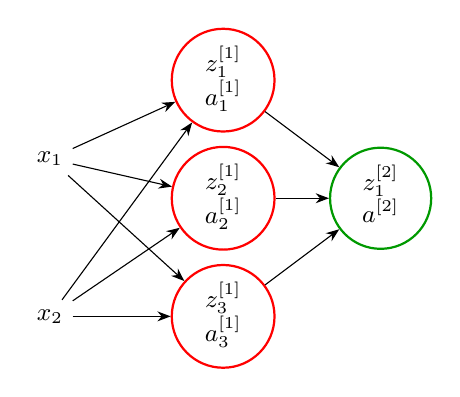
\begin{tikzpicture}[>=Stealth, node distance=1.2cm and 1.2cm, every node/.style={font=\small}, scale=1, transform shape]

% Input layer
\node (x1) at (0,3) {$x_1$};
\node (x2) at (0,1) {$x_2$};

% Hidden layer (red)
\node[circle,draw=red,thick,minimum size=1cm] (a1) at (2.2,4) {$\begin{matrix} z^{[1]}_1 \\ a^{[1]}_1 \end{matrix}$};
\node[circle,draw=red,thick,minimum size=1cm] (a2) at (2.2,2.5) {$\begin{matrix} z^{[1]}_2 \\ a^{[1]}_2 \end{matrix}$};
\node[circle,draw=red,thick,minimum size=1cm] (a3) at (2.2,1) {$\begin{matrix} z^{[1]}_3 \\ a^{[1]}_3 \end{matrix}$};

% Output layer (green)
\node[circle,draw=green!60!black,thick,minimum size=1cm] (a4) at (4.2,2.5) {$\begin{matrix} z^{[2]}_1 \\ a^{[2]} \end{matrix}$};

% Connections (input to hidden)
\draw[->] (x1) -- (a1);
\draw[->] (x1) -- (a2);
\draw[->] (x1) -- (a3);

\draw[->] (x2) -- (a1);
\draw[->] (x2) -- (a2);
\draw[->] (x2) -- (a3);

% Connections (hidden to output)
\draw[->] (a1) -- (a4);
\draw[->] (a2) -- (a4);
\draw[->] (a3) -- (a4);

\end{tikzpicture}

\vspace{1.5em}

% Equations side-by-side
\begin{minipage}{0.45\textwidth}
  \centering
  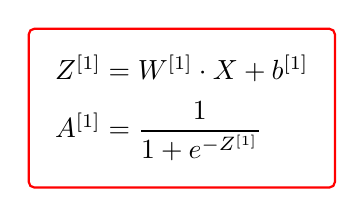
\begin{tikzpicture}
  \node[align=left] (eqs1) {
    $Z^{[1]} = W^{[1]} \cdot X + b^{[1]}$\\[0.6em]
    $A^{[1]} = \dfrac{1}{1 + e^{-Z^{[1]}}}$
  };
  \node[draw=red, thick, rounded corners=2pt, fit={(eqs1)}, inner sep=6pt] {};
  \end{tikzpicture}
\end{minipage}
\hfill
\begin{minipage}{0.45\textwidth}
  \centering
  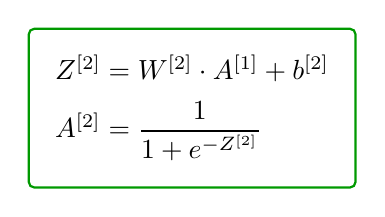
\begin{tikzpicture}
  \node[align=left] (eqs2) {
    $Z^{[2]} = W^{[2]} \cdot A^{[1]} + b^{[2]}$\\[0.6em]
    $A^{[2]} = \dfrac{1}{1 + e^{-Z^{[2]}}}$
  };
  \node[draw=green!60!black, thick, rounded corners=2pt, fit={(eqs2)}, inner sep=6pt] {};
  \end{tikzpicture}
\end{minipage}

\end{frame}
%
%..................................................................
%
\begin{frame}{Forward Propagation 3-Layer Network}

\centering
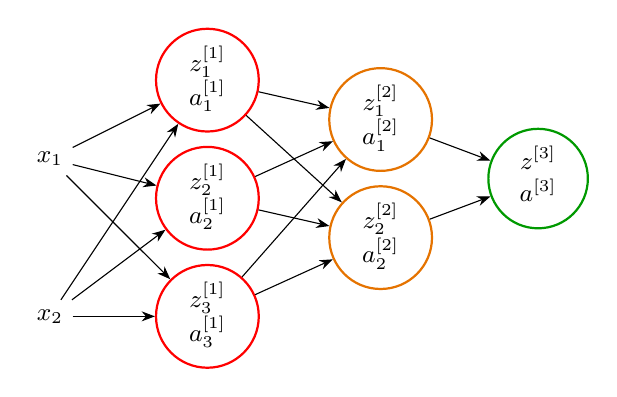
\begin{tikzpicture}[>=Stealth, node distance=1.2cm and 1.2cm, every node/.style={font=\small}, scale=1, transform shape]

% Input layer
\node (x1) at (0,3) {$x_1$};
\node (x2) at (0,1) {$x_2$};

% Hidden layer 1 (red)
\node[circle,draw=red,thick,minimum size=1cm] (h1a) at (2,4) {$\begin{matrix} z^{[1]}_1 \\ a^{[1]}_1 \end{matrix}$};
\node[circle,draw=red,thick,minimum size=1cm] (h1b) at (2,2.5) {$\begin{matrix} z^{[1]}_2 \\ a^{[1]}_2 \end{matrix}$};
\node[circle,draw=red,thick,minimum size=1cm] (h1c) at (2,1) {$\begin{matrix} z^{[1]}_3 \\ a^{[1]}_3 \end{matrix}$};

% Hidden layer 2 (orange)
\node[circle,draw=orange!90!black,thick,minimum size=1cm] (h2a) at (4.2,3.5) {$\begin{matrix} z^{[2]}_1 \\ a^{[2]}_1 \end{matrix}$};
\node[circle,draw=orange!90!black,thick,minimum size=1cm] (h2b) at (4.2,2) {$\begin{matrix} z^{[2]}_2 \\ a^{[2]}_2 \end{matrix}$};

% Output layer (green)
\node[circle,draw=green!60!black,thick,minimum size=1cm] (out) at (6.2,2.75) {$\begin{matrix} z^{[3]} \\ a^{[3]} \end{matrix}$};

% Connections: Input → Hidden 1
\foreach \i in {h1a,h1b,h1c} {
  \draw[->] (x1) -- (\i);
  \draw[->] (x2) -- (\i);
}

% Connections: Hidden 1 → Hidden 2
\foreach \i in {h1a,h1b,h1c} {
  \foreach \j in {h2a,h2b} {
    \draw[->] (\i) -- (\j);
  }
}

% Connections: Hidden 2 → Output
\draw[->] (h2a) -- (out);
\draw[->] (h2b) -- (out);

\end{tikzpicture}

\vspace{1.2em}

% Equation blocks: compact layout
\begin{minipage}{0.3\textwidth}
  \centering
  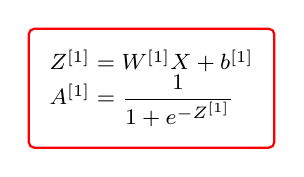
\begin{tikzpicture}
  \node[align=left, font=\footnotesize] (eqs1) {
    $Z^{[1]} = W^{[1]}X + b^{[1]}$\\
    $A^{[1]} = \dfrac{1}{1 + e^{-Z^{[1]}}}$
  };
  \node[draw=red, thick, rounded corners=2pt, fit={(eqs1)}, inner sep=4pt] {};
  \end{tikzpicture}
\end{minipage}
\hfill
\begin{minipage}{0.3\textwidth}
  \centering
  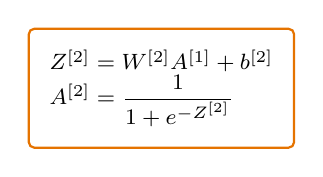
\begin{tikzpicture}
  \node[align=left, font=\footnotesize] (eqs2) {
    $Z^{[2]} = W^{[2]}A^{[1]} + b^{[2]}$\\
    $A^{[2]} = \dfrac{1}{1 + e^{-Z^{[2]}}}$
  };
  \node[draw=orange!90!black, thick, rounded corners=2pt, fit={(eqs2)}, inner sep=4pt] {};
  \end{tikzpicture}
\end{minipage}
\hfill
\begin{minipage}{0.3\textwidth}
  \centering
  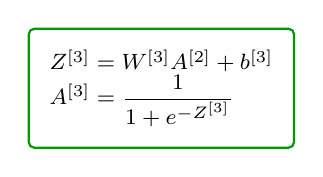
\begin{tikzpicture}
  \node[align=left, font=\footnotesize] (eqs3) {
    $Z^{[3]} = W^{[3]}A^{[2]} + b^{[3]}$\\
    $A^{[3]} = \dfrac{1}{1 + e^{-Z^{[3]}}}$
  };
  \node[draw=green!60!black, thick, rounded corners=2pt, fit={(eqs3)}, inner sep=4pt] {};
  \end{tikzpicture}
\end{minipage}

\end{frame}
%
%..................................................................
%
\begin{frame}{Backpropagation – 2-Layer Network}

\centering
% === Network Diagram ===
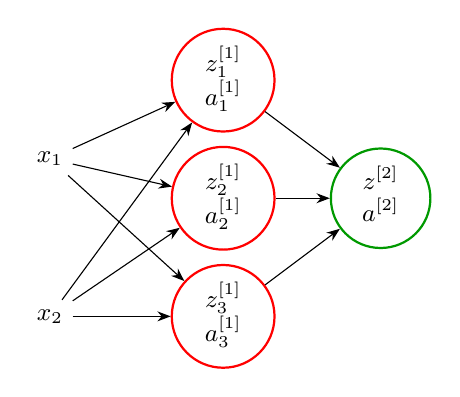
\begin{tikzpicture}[>=Stealth, node distance=1.2cm and 1.2cm, every node/.style={font=\small}, scale=1, transform shape]

% Input layer
\node (x1) at (0,3) {$x_1$};
\node (x2) at (0,1) {$x_2$};

% Hidden layer (red)
\node[circle,draw=red,thick,minimum size=1cm] (a1) at (2.2,4) {$\begin{matrix} z^{[1]}_1 \\ a^{[1]}_1 \end{matrix}$};
\node[circle,draw=red,thick,minimum size=1cm] (a2) at (2.2,2.5) {$\begin{matrix} z^{[1]}_2 \\ a^{[1]}_2 \end{matrix}$};
\node[circle,draw=red,thick,minimum size=1cm] (a3) at (2.2,1) {$\begin{matrix} z^{[1]}_3 \\ a^{[1]}_3 \end{matrix}$};

% Output layer (green)
\node[circle,draw=green!60!black,thick,minimum size=1cm] (a4) at (4.2,2.5) {$\begin{matrix} z^{[2]} \\ a^{[2]} \end{matrix}$};

% Connections (input to hidden)
\draw[->] (x1) -- (a1);
\draw[->] (x1) -- (a2);
\draw[->] (x1) -- (a3);

\draw[->] (x2) -- (a1);
\draw[->] (x2) -- (a2);
\draw[->] (x2) -- (a3);

% Connections (hidden to output)
\draw[->] (a1) -- (a4);
\draw[->] (a2) -- (a4);
\draw[->] (a3) -- (a4);

\end{tikzpicture}

\vspace{.25em}

% === Backprop Equations Below (side-by-side) ===
\begin{minipage}{0.45\textwidth}
  \centering
  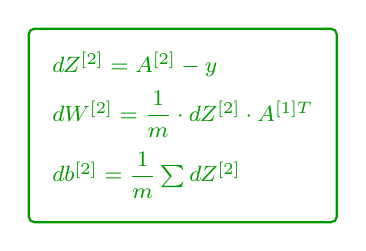
\begin{tikzpicture}
  \node[align=left, font=\footnotesize] (eqs2) {
    $\textcolor{green!60!black}{dZ^{[2]} = A^{[2]} - y}$\\[0.5em]
    $\textcolor{green!60!black}{dW^{[2]} = \dfrac{1}{m} \cdot dZ^{[2]} \cdot A^{[1]T}}$\\[0.5em]
    $\textcolor{green!60!black}{db^{[2]} = \dfrac{1}{m} \sum dZ^{[2]}}$
  };
  \node[draw=green!60!black, thick, rounded corners=2pt, fit={(eqs2)}, inner sep=5pt] {};
  \end{tikzpicture}
\end{minipage}
\hfill
\begin{minipage}{0.45\textwidth}
  \centering
  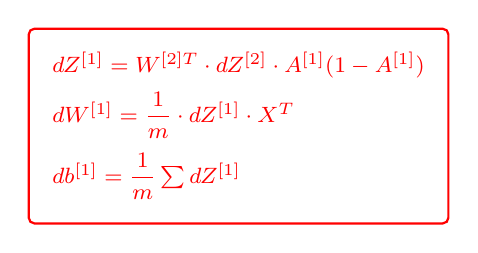
\begin{tikzpicture}
  \node[align=left, font=\footnotesize] (eqs1) {
    $\textcolor{red}{dZ^{[1]} = W^{[2]T} \cdot dZ^{[2]} \cdot A^{[1]}(1 - A^{[1]})}$\\[0.5em]
    $\textcolor{red}{dW^{[1]} = \dfrac{1}{m} \cdot dZ^{[1]} \cdot X^T}$\\[0.5em]
    $\textcolor{red}{db^{[1]} = \dfrac{1}{m} \sum dZ^{[1]}}$
  };
  \node[draw=red, thick, rounded corners=2pt, fit={(eqs1)}, inner sep=5pt] {};
  \end{tikzpicture}
\end{minipage}

\end{frame}
%
%..................................................................
%
\begin{frame}{Backpropagation – 3-Layer Network}

\centering
\vspace{-1.5cm}
% === Network Diagram ===
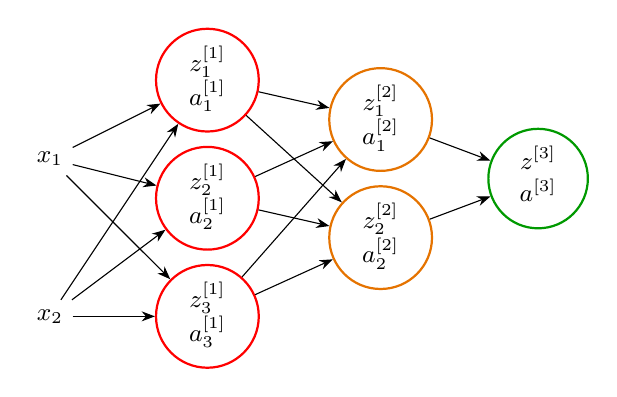
\begin{tikzpicture}[>=Stealth, node distance=1.2cm and 1.2cm, every node/.style={font=\small}, scale=1, transform shape]

% Input layer
\node (x1) at (0,3) {$x_1$};
\node (x2) at (0,1) {$x_2$};

% Hidden layer 1 (red)
\node[circle,draw=red,thick,minimum size=1cm] (h1a) at (2,4) {$\begin{matrix} z^{[1]}_1 \\ a^{[1]}_1 \end{matrix}$};
\node[circle,draw=red,thick,minimum size=1cm] (h1b) at (2,2.5) {$\begin{matrix} z^{[1]}_2 \\ a^{[1]}_2 \end{matrix}$};
\node[circle,draw=red,thick,minimum size=1cm] (h1c) at (2,1) {$\begin{matrix} z^{[1]}_3 \\ a^{[1]}_3 \end{matrix}$};

% Hidden layer 2 (orange)
\node[circle,draw=orange!90!black,thick,minimum size=1cm] (h2a) at (4.2,3.5) {$\begin{matrix} z^{[2]}_1 \\ a^{[2]}_1 \end{matrix}$};
\node[circle,draw=orange!90!black,thick,minimum size=1cm] (h2b) at (4.2,2) {$\begin{matrix} z^{[2]}_2 \\ a^{[2]}_2 \end{matrix}$};

% Output layer (green)
\node[circle,draw=green!60!black,thick,minimum size=1cm] (out) at (6.2,2.75) {$\begin{matrix} z^{[3]} \\ a^{[3]} \end{matrix}$};

% Connections: Input → Hidden 1
\foreach \i in {h1a,h1b,h1c} {
  \draw[->] (x1) -- (\i);
  \draw[->] (x2) -- (\i);
}

% Connections: Hidden 1 → Hidden 2
\foreach \i in {h1a,h1b,h1c} {
  \foreach \j in {h2a,h2b} {
    \draw[->] (\i) -- (\j);
  }
}

% Connections: Hidden 2 → Output
\draw[->] (h2a) -- (out);
\draw[->] (h2b) -- (out);

\end{tikzpicture}
% === Equation Boxes Positioned Manually Below ===
% Output layer equations (left)
\begin{textblock*}{4.2cm}(-0.5cm,6.5cm)
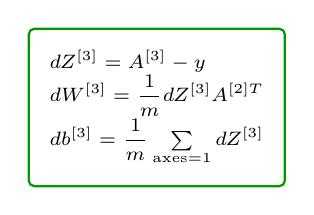
\begin{tikzpicture}
\node[align=left, font=\scriptsize] (eqs3) {
  $dZ^{[3]} = A^{[3]} - y$\\
  $dW^{[3]} = \dfrac{1}{m} dZ^{[3]} A^{[2]T}$\\
  $db^{[3]} = \dfrac{1}{m} \sum\limits_{\text{axes}=1} dZ^{[3]}$
};
\node[draw=green!60!black, thick, rounded corners=2pt, fit={(eqs3)}, inner sep=4pt] {};
\end{tikzpicture}
\end{textblock*}

% Hidden layer 2 equations (center)
\begin{textblock*}{3.4cm}(3.25cm,6.5cm)
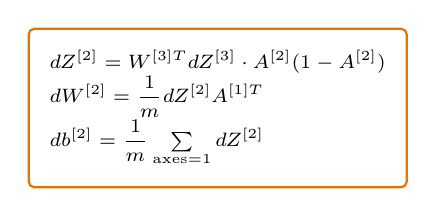
\begin{tikzpicture}
\node[align=left, font=\scriptsize] (eqs2) {
  $dZ^{[2]} = W^{[3]T} dZ^{[3]} \cdot A^{[2]}(1 - A^{[2]})$\\
  $dW^{[2]} = \dfrac{1}{m} dZ^{[2]} A^{[1]T}$\\
  $db^{[2]} = \dfrac{1}{m} \sum\limits_{\text{axes}=1} dZ^{[2]}$
};
\node[draw=orange!90!black, thick, rounded corners=2pt, fit={(eqs2)}, inner sep=4pt] {};
\end{tikzpicture}
\end{textblock*}

% Hidden layer 1 equations (right)
\begin{textblock*}{4.0cm}(8.1cm,6.5cm)
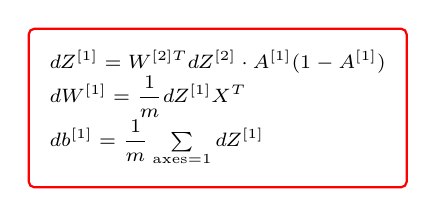
\begin{tikzpicture}
\node[align=left, font=\scriptsize] (eqs1) {
  $dZ^{[1]} = W^{[2]T} dZ^{[2]} \cdot A^{[1]}(1 - A^{[1]})$\\
  $dW^{[1]} = \dfrac{1}{m} dZ^{[1]} X^T$\\
  $db^{[1]} = \dfrac{1}{m} \sum\limits_{\text{axes}=1} dZ^{[1]}$
};
\node[draw=red, thick, rounded corners=2pt, fit={(eqs1)}, inner sep=4pt] {};
\end{tikzpicture}
\end{textblock*}

\end{frame}
%
%..................................................................
%
\begin{frame}{Backpropagation – 3-Layer Network}

% Output layer equations (top)
\begin{textblock*}{4.5cm}(0.2cm,2cm)
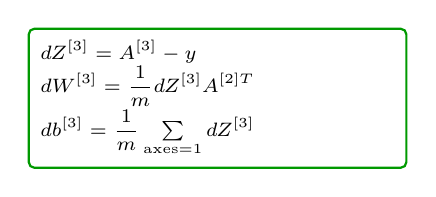
\begin{tikzpicture}
\node[inner sep=0pt] (eqs3) {
  \parbox{4.5cm}{\scriptsize
    $dZ^{[3]} = A^{[3]} - y$\\
    $dW^{[3]} = \dfrac{1}{m} dZ^{[3]} A^{[2]T}$\\
    $db^{[3]} = \dfrac{1}{m} \sum\limits_{\text{axes}=1} dZ^{[3]}$
  }
};
\node[draw=green!60!black, thick, rounded corners=2pt, fit={(eqs3)}, inner sep=4pt] {};
\end{tikzpicture}
\end{textblock*}

% Hidden layer 2 equations (middle)
\begin{textblock*}{4.5cm}(0.2cm,4.1cm)
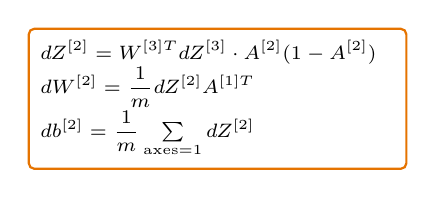
\begin{tikzpicture}
\node[inner sep=0pt] (eqs2) {
  \parbox{4.5cm}{\scriptsize
    $dZ^{[2]} = W^{[3]T} dZ^{[3]} \cdot A^{[2]}(1 - A^{[2]})$\\
    $dW^{[2]} = \dfrac{1}{m} dZ^{[2]} A^{[1]T}$\\
    $db^{[2]} = \dfrac{1}{m} \sum\limits_{\text{axes}=1} dZ^{[2]}$
  }
};
\node[draw=orange!90!black, thick, rounded corners=2pt, fit={(eqs2)}, inner sep=4pt] {};
\end{tikzpicture}
\end{textblock*}

% Hidden layer 1 equations (bottom)
\begin{textblock*}{4.5cm}(0.2cm,6.25cm)
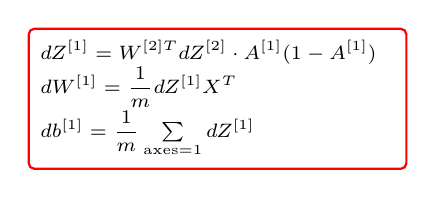
\begin{tikzpicture}
\node[inner sep=0pt] (eqs1) {
  \parbox{4.5cm}{\scriptsize
    $dZ^{[1]} = W^{[2]T} dZ^{[2]} \cdot A^{[1]}(1 - A^{[1]})$\\
    $dW^{[1]} = \dfrac{1}{m} dZ^{[1]} X^T$\\
    $db^{[1]} = \dfrac{1}{m} \sum\limits_{\text{axes}=1} dZ^{[1]}$
  }
};
\node[draw=red, thick, rounded corners=2pt, fit={(eqs1)}, inner sep=4pt] {};
\end{tikzpicture}
\end{textblock*}

\begin{textblock*}{6.5cm}(5.5cm,3cm)
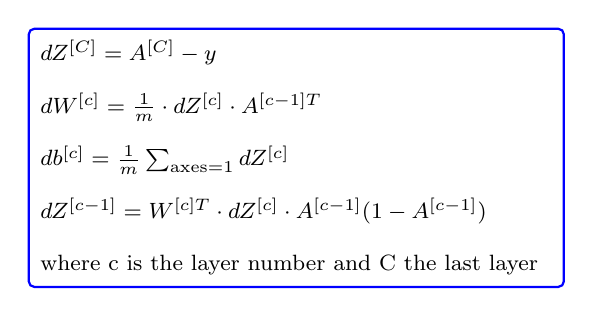
\begin{tikzpicture}
\node[inner sep=0pt] (eqs1) {
  \parbox{6.5cm}{\footnotesize
	$dZ^{[C]} = A^{[C]} - y$\\
	$ $\\ 
    $dW^{[c]} = \frac{1}{m} \cdot dZ^{[c]} \cdot A^{[c-1]T}$\\
    $ $\\
    $db^{[c]} = \frac{1}{m} \sum_{\text{axes}=1} dZ^{[c]}$\\
    $ $\\
    $dZ^{[c-1]} = W^{[c]T} \cdot dZ^{[c]} \cdot A^{[c-1]}(1 - A^{[c-1]})$\\
    $ $\\
    $\text{where c is the layer number and C the last layer} $
  }
};
\node[draw=blue, thick, rounded corners=2pt, fit={(eqs1)}, inner sep=4pt] {};
\end{tikzpicture}
\end{textblock*}

\end{frame}
%
%..................................................................
%
\begin{frame}[fragile]{From Two Layers to a General Deep Network}
\framesubtitle{Parameterizing a Network of Arbitrary Depth}

{\small The 2-layer network used \textbf{named variables}: $W^{[1]}\!, b^{[1]}\!, W^{[2]}\!, b^{[2]}$. To generalize to $C$ layers, we store all parameters in a single \textbf{dictionary} indexed by layer number $c = 1, \dots, C$\,:}

\begin{block}{\small Architecture specification}
{\small A Python list defines the full topology:}
\begin{center}
\texttt{\small dimensions = [$n_0$, $n_1$, $n_2$, \dots, $n_C$]}
\end{center}
{\small where $n_0$ = input features, $n_C$ = output (1 for binary).}
\end{block}

{\small\textbf{Key change:} every hard-coded ``\texttt{W1}, \texttt{W2}'' becomes a \textbf{loop} over $c$. For instance, the 2-layer \texttt{W1~=~random(n1,~n0);~W2~=~random(n2,~n1)} becomes simply \texttt{for~c~in~1..C:~W\{c\}~=~random(n$_c$,~n$_{c-1}$)}.}

\end{frame}
%
%..................................................................
%
\begin{frame}[fragile]{From Two Layers to a General Deep Network}
\framesubtitle{Parameterizing a Network of Arbitrary Depth}

\textbf{Initialization --- generalized}
\begin{lstlisting}
def initialization(dimensions):
    parameters = {}
    C = len(dimensions)
    for c in range(1, C):
        parameters['W' + str(c)] = \
            np.random.randn(
                dimensions[c], 
                dimensions[c-1])
        parameters['b' + str(c)] = \
            np.random.randn(
                dimensions[c], 1)
    return parameters
\end{lstlisting}
\end{frame}
%
%..................................................................
%
\begin{frame}[fragile]{From Two Layers to a General Deep Network}
\colorbox{blue!8}{\parbox{0.92\linewidth}{\normalsize
\textbf{Example:} \texttt{dimensions = [2, 16, 32, 1]}\\[1pt]
$\Rightarrow$ $C=3$ layers, with:\\
\quad $W^{[1]} \in \mathbb{R}^{16\times 2}$, \;
$W^{[2]} \in \mathbb{R}^{32\times 16}$, \;
$W^{[3]} \in \mathbb{R}^{1\times 32}$}}

\end{frame}
%
%..................................................................
%
\begin{frame}[fragile]{Forward and Backward Propagation --- Generalized}
\framesubtitle{One Loop Replaces All Layer-Specific Equations}

\textbf{\small Forward propagation}
{\small Set $A^{[0]} = X$, then for $c = 1, \dots, C$:}
{\small\color{layer1violet}
\[
\boxed{Z^{[c]} = W^{[c]} A^{[c-1]} + b^{[c]}, \quad A^{[c]} = \sigma(Z^{[c]})}
\]
}
\small
\begin{lstlisting}
def forward_propagation(X, parameters):
    activations = {'A0': X}
    C = len(parameters) // 2
    for c in range(1, C + 1):
        Z = parameters['W'+str(c)].dot(
              activations['A'+str(c-1)]) \
              + parameters['b'+str(c)]
        activations['A'+str(c)] = \
              1 / (1 + np.exp(-Z))
    return activations
\end{lstlisting}

%\colorbox{blue!8}{\parbox{0.92\linewidth}{\scriptsize
%\textbf{Note:} The 2-layer version had two explicit blocks of code for $Z^{[1]}\!,A^{[1]}$ and $Z^{[2]}\!,A^{[2]}$. Here a single \texttt{for} loop handles any depth.}}

\end{frame}
%
%..................................................................
%
\begin{frame}[fragile]{Forward and Backward Propagation --- Generalized}
\framesubtitle{One Loop Replaces All Layer-Specific Equations}

\textbf{\small Backpropagation}

{\small Initialize $dZ^{[C]} = A^{[C]} - y$, then for $c = C, \dots, 1$:}

{\small
\[
\boxed{dW^{[c]} \!=\! \tfrac{1}{m} dZ^{[c]} {A^{[c-1]}}^{\!\top}\!, \;\; db^{[c]} \!=\! \tfrac{1}{m} \textstyle\sum dZ^{[c]}}
\]
}
{\small If $c > 1$: \; ${\color{layer1violet}dZ^{[c-1]} = {W^{[c]}}^{\!\top} dZ^{[c]} \odot A^{[c-1]}\!(1 - A^{[c-1]})}$}

{\lstset{basicstyle=\ttfamily\fontsize{5.5}{7}\selectfont}
\begin{lstlisting}
def back_propagation(y, activations, parameters):
    m = y.shape[1]
    C = len(parameters) // 2
    dZ = activations['A'+str(C)] - y
    gradients = {}
    for c in reversed(range(1, C+1)):
        gradients['dW'+str(c)] = \
            1/m * dZ.dot(activations['A'+str(c-1)].T)
        gradients['db'+str(c)] = \
            1/m * np.sum(dZ, axis=1, keepdims=True)
        if c > 1:
            dZ = parameters['W'+str(c)].T.dot(dZ) \
                 * activations['A'+str(c-1)] \
                 * (1 - activations['A'+str(c-1)])
    return gradients
\end{lstlisting}
}

\end{frame}
%
%..................................................................
%
\begin{frame}[fragile]{Parameter Update and Training Loop}
\framesubtitle{Completing the Generalized Training Algorithm}

\textbf{\small Update rule --- generalized}
{\small The update applies the \textbf{same rule at every layer}:}
{\small
\[
\boxed{W^{[c]} \leftarrow W^{[c]} - \eta\, dW^{[c]}, \quad b^{[c]} \leftarrow b^{[c]} - \eta\, db^{[c]}}
\]
}
\begin{lstlisting}
def update(gradients, parameters, 
           learning_rate):
    C = len(parameters) // 2
    for c in range(1, C + 1):
        parameters['W' + str(c)] -= \
            learning_rate * \
            gradients['dW' + str(c)]
        parameters['b' + str(c)] -= \
            learning_rate * \
            gradients['db' + str(c)]
    return parameters
\end{lstlisting}

\vspace{0.05cm}

{\scriptsize\colorbox{blue!8}{\parbox{0.92\linewidth}{%
\textbf{Predict:} run \texttt{forward\_propagation}, read $A^{[C]} \!\geq\! 0.5$. Depth extracted via \texttt{len(parameters)//2}.}}}

\end{frame}
%
%..................................................................
%
\begin{frame}[fragile]{Parameter Update and Training Loop}
\framesubtitle{Completing the Generalized Training Algorithm}

\textbf{\small Training loop}
\begin{lstlisting}
for i in range(n_iter):
    activations = forward_propagation(
                       X_train, parameters)
    gradients = back_propagation(
                       y_train, activations,
                       parameters)
    parameters = update(
                       gradients, parameters,
                       learning_rate)
\end{lstlisting}
\end{frame}
%
%..................................................................
%
\begin{frame}[fragile]{Parameter Update and Training Loop}
\framesubtitle{Completing the Generalized Training Algorithm}
\textbf{\small What changed from the 2-layer version?}

\vspace{0.5cm}
{\normalsize
\renewcommand{\arraystretch}{1.05}
\begin{tabular}{@{}p{4cm}@{\;\;}p{4cm}@{\;\;}p{4cm}@{}}
\textbf{Component} & \textbf{2-layer} & \textbf{$C$-layer} \\
\hline
Architecture & hard-coded & \texttt{dimensions} list \\
Parameters & W1,b1,W2,b2 & dictionary \\
Forward pass & 2 explicit eqs. & \texttt{for c in 1..C} \\
Backprop & 2 explicit eqs. & \texttt{for c in C..1} \\
Update & 4 assignments & \texttt{for c in 1..C} \\
Training loop & \multicolumn{2}{c}{\textbf{identical}} \\
\end{tabular}
}
\end{frame}
%
%..................................................................
%
% Slide 1: Main training challenge
\begin{frame}{A Key Challenge in Deep Learning}

\begin{itemize}
    \item As networks get deeper, training becomes more difficult.
    \item A core problem: \textbf{gradients may vanish or explode} during backpropagation.
    \item This makes learning:
    \begin{itemize}
        \item Very slow (vanishing gradients)
        \item Unstable (exploding gradients)
    \end{itemize}
\end{itemize}

\vspace{0.3cm}
\begin{block}{\textbf{Why it happens}}
In backpropagation, the gradient is computed through repeated multiplication.
For deep networks, this can cause gradients to shrink or grow exponentially.
\end{block}

\end{frame}
%
%..................................................................
%
% Slide 2: Vanishing gradients
\begin{frame}{Vanishing Gradients}

\begin{itemize}
    \item Occurs when gradients become \textbf{very small} as they flow backward.
    \item Common when using the \textbf{sigmoid} or \textbf{tanh} activation functions.
    \item Leads to:
    \begin{itemize}
        \item Neurons in early layers learning extremely slowly.
        \item Very flat loss surfaces.
    \end{itemize}
\end{itemize}

\vspace{0.3cm}
\textbf{Mathematical Insight}
\begin{block}{}
Derivatives of sigmoid are always \( < 0.25 \), and repeated multiplication in deep networks makes gradients vanish.
\end{block}

\end{frame}
%
%..................................................................
%
% Slide 3: Exploding Gradients
\begin{frame}{Exploding Gradients}

\begin{itemize}
    \item Opposite of vanishing: gradients become \textbf{very large}.
    \item Causes:
    \begin{itemize}
        \item Unstable weight updates
        \item Diverging loss
        \item Numerical overflow (NaNs)
    \end{itemize}
    \item More common in networks with:
    \begin{itemize}
        \item Poor initialization
        \item Large learning rates
    \end{itemize}
\end{itemize}

\vspace{0.3cm}
\textbf{Symptom}
\begin{block}{}
Training loss oscillates wildly or becomes NaN.
\end{block}

\end{frame}
%
%..................................................................
%
% Slide 4: How to Deal with It
\begin{frame}{How to Address Gradient Issues}

\begin{itemize}
    \item \textbf{Use better activation functions:}
    \begin{itemize}
        \item ReLU, Leaky ReLU reduce vanishing gradient problems
    \end{itemize}
    \item \textbf{Initialize weights carefully:}
    \begin{itemize}
        \item Xavier (Glorot) initialization
        \item He initialization (for ReLU)
    \end{itemize}
    \item \textbf{Apply normalization:}
    \begin{itemize}
        \item Batch Normalization standardizes activations layer-by-layer
    \end{itemize}
    \item \textbf{Use gradient clipping:}
    \begin{itemize}
        \item Limit the norm of gradients to prevent explosion
    \end{itemize}
\end{itemize}

\vspace{0.3cm}
\textbf{Takeaway}
\begin{block}{}
Deep learning is powerful, but requires careful training design to avoid gradient instability.
\end{block}

\end{frame}
%______________________________________________________________________________
%
\subsection{Activation Functions Beyond the Sigmoid}
%______________________________________________________________________________
%
\begin{frame}{Why the Sigmoid Is Not Enough}

We have used the sigmoid $\sigma(z) = \frac{1}{1+e^{-z}}$ throughout.

\medskip
\textbf{Problems in deep networks:}
\begin{itemize}
    \item \textbf{Vanishing gradients:} $\sigma'(z) \leq 0.25$ always. In a network with $L$ layers, gradients shrink as $\sim (0.25)^L$.
    \item \textbf{Not zero-centered:} outputs are in $(0,1)$, causing zig-zag updates.
    \item \textbf{Saturation:} for large $|z|$, the gradient is nearly zero $\Rightarrow$ neurons stop learning.
\end{itemize}

\vspace{0.3cm}
\begin{alertblock}{Key insight}
Modern deep learning replaces the sigmoid with activation functions that do \textbf{not} suffer from these issues.
\end{alertblock}
\end{frame}
%
%..................................................................
%
\begin{frame}{The ReLU Activation}

The \textbf{Rectified Linear Unit} (Nair \& Hinton, 2010):
\[
g(z) = \max(z, 0)
\]

\begin{columns}
\begin{column}{0.48\textwidth}
\textbf{Advantages:}
\begin{itemize}
    \item Gradient is $1$ for $z>0$ $\Rightarrow$ no vanishing gradient
    \item Very fast to compute
    \item Induces \textbf{sparsity}: negative pre-activations are set to zero
    \item Empirically the most widely used activation
\end{itemize}
\end{column}
\begin{column}{0.48\textwidth}
\textbf{Derivative:}
\[
g'(z) = \begin{cases} 1 & z > 0 \\ 0 & z < 0 \end{cases}
\]
\textbf{Limitation:} ``dead neurons'' --- if $z < 0$ for all training inputs, the gradient is permanently zero.
\end{column}
\end{columns}

\end{frame}
%
%..................................................................
%
\begin{frame}{ReLU Variants}
\footnotesize
\begin{block}{Leaky ReLU (Maas et al., 2013)}
\[
g(z) = \begin{cases} z & z > 0 \\ \alpha z & z \leq 0 \end{cases}
\quad \text{with } \alpha \approx 0.01
\]
Prevents dead neurons by allowing a small gradient when $z < 0$.
\end{block}

\begin{block}{ELU --- Exponential Linear Unit (Clevert et al., 2015)}
\[
g(z) = \begin{cases} z & z > 0 \\ \alpha(e^z - 1) & z \leq 0 \end{cases}
\]
Smooth approximation that pushes mean activations closer to zero.
\end{block}

\begin{block}{Swish / SiLU (Ramachandran et al., 2017)}
\[
g(z) = z \cdot \sigma(z)
\]
Smooth, non-monotonic. Often outperforms ReLU in very deep networks.
\end{block}
\end{frame}
%
%..................................................................
%
\begin{frame}{Choosing an Activation Function --- Practical Guidelines}

\begin{center}
\renewcommand{\arraystretch}{1.4}
\begin{tabular}{l c c c}
\hline
\textbf{Activation} & \textbf{Range} & \textbf{Vanishing?} & \textbf{Typical use} \\
\hline
Sigmoid $\sigma(z)$ & $(0,1)$ & Yes & Output layer (binary) \\
Tanh & $(-1,1)$ & Yes & Recurrent networks \\
\textbf{ReLU} & $[0,\infty)$ & No & \textbf{Hidden layers (default)} \\
Leaky ReLU & $(-\infty,\infty)$ & No & Hidden layers \\
Softmax & $(0,1)^K$ & --- & Output (multiclass) \\
Linear & $(-\infty,\infty)$ & No & Output (regression) \\
\hline
\end{tabular}
\end{center}

\vspace{0.3cm}
\footnotesize
\textbf{Rule of thumb:}
\begin{itemize}
    \item \textbf{Hidden layers:} start with ReLU
    \item \textbf{Output layer:} match the problem (sigmoid for binary, softmax for multiclass, linear for regression)
\end{itemize}
\end{frame}
%______________________________________________________________________________
%
\subsection{Stochastic Optimization}
%______________________________________________________________________________
%
\begin{frame}{From Full-Batch to Stochastic Gradient Descent}
\small
So far we computed the gradient over \textbf{all} $m$ training examples:
\[
\theta \leftarrow \theta - \eta \nabla_\theta \mathcal{L}(\theta) = \theta - \eta \cdot \frac{1}{m}\sum_{i=1}^m \nabla_\theta \ell_i(\theta)
\]

\textbf{Problem:} when $m$ is very large, each gradient step is extremely expensive.

\medskip
\textbf{Example from finance:} In Gu, Kelly \& Xiu (2019), the dataset has ${\sim}30{,}000$ stocks over 720 months. Computing the full gradient at each step is prohibitive.

\vspace{0.3cm}
\begin{alertblock}{Key idea: Stochastic Gradient Descent (SGD)}
Approximate the gradient using a small random \textbf{mini-batch} $\mathcal{B}_t \subset \{1,\ldots,m\}$:
\[
\theta \leftarrow \theta - \eta \cdot \frac{1}{|\mathcal{B}_t|}\sum_{i \in \mathcal{B}_t} \nabla_\theta \ell_i(\theta)
\]
\end{alertblock}
\end{frame}
%
%..................................................................
%
\begin{frame}{Mini-Batch Gradient Descent}
\small
\textbf{Three regimes:}

\medskip
\begin{center}
\renewcommand{\arraystretch}{1.3}
\begin{tabular}{l c l}
\hline
\textbf{Method} & \textbf{Batch size} & \textbf{Trade-off} \\
\hline
Full-batch GD & $|\mathcal{B}| = m$ & Accurate but slow \\
Pure SGD & $|\mathcal{B}| = 1$ & Fast but very noisy \\
\textbf{Mini-batch SGD} & $|\mathcal{B}| \in [32, 512]$ & \textbf{Best compromise} \\
\hline
\end{tabular}
\end{center}

\vspace{0.4cm}
\textbf{Training protocol (one epoch = one pass through the data):}
\begin{enumerate}
    \item Shuffle the training set randomly
    \item Split into mini-batches of size $b$
    \item For each mini-batch: compute gradient, update $\theta$
    \item Repeat for multiple epochs
\end{enumerate}

\medskip
Mini-batch SGD introduces \textbf{noise} in the gradient estimate, which can actually help escape local minima.
\end{frame}
%
%..................................................................
%
\begin{frame}{The Problem with a Fixed Learning Rate}
\small
In SGD with a constant learning rate $\eta$:

\begin{itemize}
    \item \textbf{Too large $\eta$:} the optimizer overshoots and diverges
    \item \textbf{Too small $\eta$:} convergence is extremely slow
    \item Near the minimum, the \textbf{noise dominates} the gradient signal $\Rightarrow$ the optimizer oscillates instead of converging
\end{itemize}

\vspace{0.3cm}
\textbf{Desired behavior:}
\begin{itemize}
    \item Take large steps early in training (when far from the optimum)
    \item Take smaller steps later (to fine-tune)
    \item Adapt the step size \textbf{per-parameter}, since different weights may need different learning rates
\end{itemize}

\vspace{0.3cm}
\textbf{Solution:} \emph{adaptive} optimizers that adjust the learning rate automatically.
\end{frame}
%
%..................................................................
%
\begin{frame}{The Adam Optimizer (Kingma \& Ba, 2014)}
\small
\textbf{Adam} (Adaptive Moment Estimation) combines two ideas:
\begin{itemize}
    \item \textbf{Momentum:} use a running average of past gradients (1st moment)
    \item \textbf{Adaptive learning rate:} scale by a running average of squared gradients (2nd moment)
\end{itemize}

\medskip
\textbf{Update rules} at iteration $t$:
\begin{align*}
g_t &= \nabla_\theta \mathcal{L}(\theta_{t-1}) && \text{(gradient on mini-batch)}\\
m_t &= \beta_1 m_{t-1} + (1 - \beta_1) g_t && \text{(1st moment estimate)}\\
v_t &= \beta_2 v_{t-1} + (1 - \beta_2) g_t^2 && \text{(2nd moment estimate)}\\
\hat{m}_t &= m_t / (1 - \beta_1^t) && \text{(bias correction)}\\
\hat{v}_t &= v_t / (1 - \beta_2^t) && \text{(bias correction)}\\
\theta_t &= \theta_{t-1} - \alpha \cdot \hat{m}_t / (\sqrt{\hat{v}_t} + \epsilon) && \text{(parameter update)}
\end{align*}

\medskip
\textbf{Default hyperparameters:} $\beta_1 = 0.9$, $\beta_2 = 0.999$, $\epsilon = 10^{-8}$.
\end{frame}
%
%..................................................................
%
\begin{frame}{Why Adam Works Well}

\begin{columns}
\begin{column}{0.55\textwidth}
\textbf{Momentum ($m_t$):}
\begin{itemize}
    \item Smooths out noisy gradients
    \item Accelerates in consistent directions
    \item Like a ball rolling downhill with inertia
\end{itemize}

\medskip
\textbf{Adaptive scaling ($v_t$):}
\begin{itemize}
    \item Parameters with large gradients get \emph{smaller} updates
    \item Parameters with small gradients get \emph{larger} updates
    \item Effectively uses a different learning rate for each parameter
\end{itemize}
\end{column}
\begin{column}{0.42\textwidth}
\begin{block}{Comparison}
\small
\begin{tabular}{l l}
\textbf{SGD} & One $\eta$ for all \\
\textbf{Momentum} & + smoothing \\
\textbf{RMSProp} & + adaptive $\eta$ \\
\textbf{Adam} & All combined \\
\end{tabular}
\end{block}

\vspace{0.3cm}
\begin{alertblock}{In practice}
Adam is the \textbf{default optimizer} in most deep learning applications, including Gu, Kelly \& Xiu (2019).
\end{alertblock}
\end{column}
\end{columns}
\end{frame}
%______________________________________________________________________________
%
\subsection{Regularization}
%______________________________________________________________________________
%
\begin{frame}{The Overfitting Problem}

\textbf{Overfitting} occurs when a model fits the \textbf{noise} in the training data, rather than the underlying signal.

\begin{columns}
\begin{column}{0.50\textwidth}
\textbf{Symptoms:}
\begin{itemize}
    \item Training loss keeps decreasing
    \item Validation loss starts \textbf{increasing}
    \item Large gap between train/test performance
\end{itemize}

\medskip
\textbf{Why neural networks are prone:}
\begin{itemize}
    \item Many parameters (often millions)
    \item High model capacity
    \item Can memorize training data
\end{itemize}
\end{column}
\begin{column}{0.46\textwidth}
\begin{center}
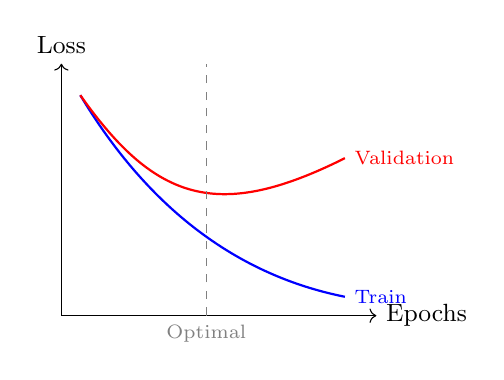
\begin{tikzpicture}[scale=0.8]
\draw[->] (0,0) -- (5,0) node[right] {\small Epochs};
\draw[->] (0,0) -- (0,4) node[above] {\small Loss};
\draw[blue, thick] (0.3,3.5) .. controls (1.5,1.5) and (3,0.6) .. (4.5,0.3);
\node[blue, right] at (4.5,0.3) {\scriptsize Train};
\draw[red, thick] (0.3,3.5) .. controls (1.5,1.8) and (2.5,1.5) .. (4.5,2.5);
\node[red, right] at (4.5,2.5) {\scriptsize Validation};
\draw[dashed, gray] (2.3,0) -- (2.3,4);
\node[gray, below] at (2.3,0) {\scriptsize Optimal};
\end{tikzpicture}
\end{center}
\end{column}
\end{columns}

\vspace{0.3cm}
\textbf{Regularization} = any technique that improves generalization by constraining model complexity.
\end{frame}
%
%..................................................................
%
\begin{frame}{$\ell_1$ Penalization (LASSO)}

Append a penalty to the loss function that discourages large weights:
\[
\boxed{\mathcal{L}_{\text{reg}}(\theta) = \mathcal{L}(\theta) + \lambda \sum_j |\theta_j|}
\]

\begin{itemize}
    \item The penalty $\lambda \sum_j |\theta_j|$ is called \textbf{LASSO} ($\ell_1$) regularization
    \item $\lambda \geq 0$ is a hyperparameter controlling regularization strength
    \item \textbf{Key property:} the geometry of the $\ell_1$ ball sets some weights to \textbf{exactly zero} $\Rightarrow$ \textbf{sparsity}
\end{itemize}

\vspace{0.3cm}
\textbf{Effect:}
\begin{itemize}
    \item Irrelevant features are automatically discarded
    \item The model becomes simpler and more interpretable
    \item Out-of-sample performance improves by reducing noise fitting
\end{itemize}

\end{frame}
%
%..................................................................
%
\begin{frame}{$\ell_1$ vs $\ell_2$ Penalization}
\begin{columns}
\begin{column}{0.48\textwidth}
\textbf{LASSO / $\ell_1$:}
\[
\phi(\theta) = \lambda \sum_j |\theta_j|
\]
\begin{itemize}
    \item Produces \textbf{sparse} solutions
    \item Feature selection built-in
    \item Non-differentiable at $\theta_j = 0$
\end{itemize}
\end{column}
\begin{column}{0.48\textwidth}
\textbf{Ridge / $\ell_2$:}
\[
\phi(\theta) = \lambda \sum_j \theta_j^2
\]
\begin{itemize}
    \item Shrinks weights toward zero but \textbf{never exactly zero}
    \item Differentiable everywhere
    \item Penalizes large weights more
\end{itemize}
\end{column}
\end{columns}
\end{frame}
%
%..................................................................
%
\begin{frame}{$\ell_1$ vs $\ell_2$ Penalization}
\begin{center}
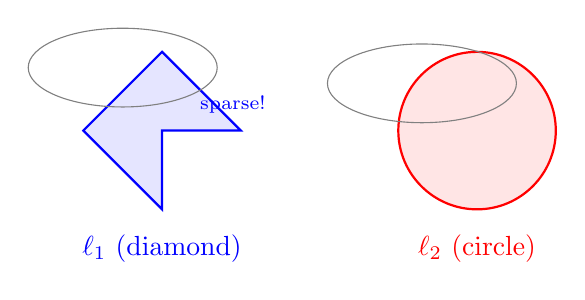
\begin{tikzpicture}[scale=1.0]
% L1 ball
\draw[blue, thick, fill=blue!10] (0,0) -- (1,0) -- (0,1) -- (-1,0) -- (0,-1) -- cycle;
\node[blue] at (0,-1.5) {$\ell_1$ (diamond)};
% L2 ball
\draw[red, thick, fill=red!10] (4,0) circle (1);
\node[red] at (4,-1.5) {$\ell_2$ (circle)};
% Contour lines (ellipses) for L1
\draw[gray, thin] (-0.5,0.8) ellipse (1.2 and 0.5);
% Corner annotation
\node[blue, above] at (0.9,0.1) {\scriptsize sparse!};
% Contour lines (ellipses) for L2
\draw[gray, thin] (3.3,0.6) ellipse (1.2 and 0.5);
\end{tikzpicture}
\end{center}

\vspace{0.3cm}

The $\ell_1$ constraint set has \textbf{corners} on the axes, where some coordinates are exactly zero. The $\ell_2$ constraint set is smooth $\Rightarrow$ solutions are rarely exactly sparse.
\end{frame}
%
%..................................................................
%
\begin{frame}{Early Stopping}
\textbf{Idea:} Monitor the validation loss during training and \textbf{stop before the model overfits.}

\medskip
\textbf{Algorithm:}
\begin{enumerate}
    \item Set a \textbf{patience} parameter $p$ and initialize $j = 0$
    \item At each training step, evaluate the validation loss $\mathcal{L}'$
    \item If $\mathcal{L}' < \mathcal{L}^*_{\text{best}}$: update the best model, reset $j \leftarrow 0$
    \item Otherwise: $j \leftarrow j + 1$
    \item \textbf{Stop} when $j = p$ (no improvement for $p$ consecutive checks)
    \item Return the parameters $\theta^*$ corresponding to the best validation loss
\end{enumerate}
\end{frame}
%
%..................................................................
%
\begin{frame}{Early Stopping}
\textbf{Why it works:}
\begin{itemize}
    \item Training starts from small random weights (near-zero)
    \item Each gradient step moves $\theta$ away from zero to reduce the training loss
    \item Stopping early keeps $\theta$ close to zero $\Rightarrow$ equivalent to \textbf{implicit $\ell_2$ regularization}
\end{itemize}

\vspace{0.2cm}
\begin{block}{Advantage over explicit penalization}
Early stopping achieves regularization at \textbf{much lower computational cost}: no need to tune $\lambda$ or compute penalty gradients.
\end{block}
\end{frame}
%
%..................................................................
%
\begin{frame}{Batch Normalization (Ioffe \& Szegedy, 2015)}

\textbf{Problem:} As training progresses, the distribution of inputs to each hidden layer shifts (\textbf{internal covariate shift}). This makes training unstable, especially in deep networks.

\medskip
\textbf{Solution:} For each mini-batch and each hidden layer, normalize activations:
\[
\mu_{\mathcal{B}} = \frac{1}{N}\sum_{i=1}^N x_i, \qquad
\sigma^2_{\mathcal{B}} = \frac{1}{N}\sum_{i=1}^N (x_i - \mu_{\mathcal{B}})^2
\]
\[
\hat{x}_i = \frac{x_i - \mu_{\mathcal{B}}}{\sqrt{\sigma^2_{\mathcal{B}} + \epsilon}}
\]
\[
\boxed{y_i = \gamma \hat{x}_i + \beta}
\]

where $\gamma$ and $\beta$ are \textbf{learnable} scale and shift parameters.
\end{frame}
%
%..................................................................
%
\begin{frame}{Batch Normalization (Ioffe \& Szegedy, 2015)}
\textbf{Benefits:}
\begin{itemize}
    \item Stabilizes and \textbf{accelerates} training (allows higher learning rates)
    \item Acts as a mild regularizer
    \item Reduces sensitivity to weight initialization
\end{itemize}
\end{frame}
%
%..................................................................
%
\begin{frame}{Ensemble Methods}

\textbf{Problem:} Neural network optimization is non-convex. Different random initializations can lead to \textbf{different local optima}, each with different predictions.

\medskip
\textbf{Solution:} Train multiple networks with different random seeds, and average their predictions:
\[
\hat{y}_{\text{ensemble}} = \frac{1}{S}\sum_{s=1}^S \hat{y}^{(s)}
\]

\textbf{Why it works:}
\begin{itemize}
    \item Individual models make different errors
    \item Averaging \textbf{reduces variance} without increasing bias
    \item The ensemble is more \textbf{stable} and reliable than any single model
\end{itemize}
\end{frame}
%
%..................................................................
%
\begin{frame}{Ensemble Methods}
\vspace{0.3cm}
\begin{block}{In Gu, Kelly \& Xiu (2019)}
They use $S = 10$ random seeds for each model configuration and average the predictions. This is their third regularization technique, alongside $\ell_1$ penalization and early stopping.
\end{block}
\end{frame}
%
%..................................................................
%
\begin{frame}{Training, Validation, and Testing}
\small
\textbf{The three-way data split} is essential for reliable model evaluation:

\medskip
\begin{center}
\renewcommand{\arraystretch}{1.4}
\begin{tabular}{l p{4cm} p{5cm}}
\hline
\textbf{Sample} & \textbf{Purpose} & \textbf{What is optimized} \\
\hline
\textbf{Training} & Estimate model parameters $\theta$ & Weights $W$, biases $b$ \\
\textbf{Validation} & Tune hyperparameters & $\lambda$, learning rate, architecture \\
\textbf{Testing} & Final, unbiased evaluation & Nothing --- report results only \\
\hline
\end{tabular}
\end{center}

\vspace{0.3cm}
\textbf{Critical:} The test set must \textbf{never} influence any modeling decision.

\medskip
\textbf{For time series data} (as in asset pricing), the split must respect temporal ordering:
\begin{itemize}
    \item No future data leaks into the training set
    \item Expanding or rolling windows are preferred over random splits
\end{itemize}
\end{frame}
%
%..................................................................
%
\begin{frame}{Training, Validation, and Testing}

\begin{block}{In Gu, Kelly \& Xiu (2019)}
Training: 1957--1974, Validation: 1975--1986, Testing: 1987--2016 (30 years, purely out-of-sample). Models are refitted annually with an expanding training window.
\end{block}
\end{frame}
%
%..................................................................
%
\begin{frame}{Summary: The Deep Learning Toolkit}

Putting it all together --- the essential tools for training deep networks:

\vspace{0.3cm}
\begin{center}
\renewcommand{\arraystretch}{1.4}
\begin{tabular}{l l l}
\hline
\textbf{Component} & \textbf{Default choice} & \textbf{Role} \\
\hline
Activation (hidden) & ReLU & Nonlinearity without vanishing gradients \\
Activation (output) & Linear / Sigmoid & Task-dependent \\
Loss function & MSE / Cross-entropy & Measures prediction error \\
Optimizer & Adam & Adaptive learning rates \\
$\ell_1$ / $\ell_2$ penalty & LASSO / Ridge & Explicit weight regularization \\
Early stopping & Patience-based & Implicit regularization \\
Batch normalization & Per-layer & Stabilizes training \\
Ensemble & Multiple seeds & Reduces variance \\
\hline
\end{tabular}
\end{center}
\end{frame}
%______________________________________________________________________________
%
\section{Conclusions}
%______________________________________________________________________________
%
\begin{frame}
\frametitle{Conclusions}
\framesubtitle{Recap: What We Learned}

\textbf{Part I --- From the Perceptron to Backpropagation:}
\begin{itemize}
    \item The historical perceptron (step activation, mistake-driven) vs.\ modern differentiable models
    \item Multi-layer networks as \textbf{learned representations}: $x \to h(x) \to y$
    \item Backpropagation = systematic application of the chain rule to compute $\nabla_\theta \mathcal{L}$
\end{itemize}

\medskip
\textbf{Part II --- The Modern Deep Learning Toolkit:}
\begin{itemize}
    \item \textbf{Activation functions:} ReLU $g(z) = \max(z,0)$ solves the vanishing gradient problem
    \item \textbf{Optimization:} SGD on mini-batches $\to$ Adam (adaptive moments)
    \item \textbf{Regularization:} $\ell_1$ (LASSO) for sparsity, early stopping, batch normalization, ensemble averaging
    \item \textbf{Evaluation:} train / validation / test split with temporal ordering for financial data
\end{itemize}

\end{frame}
%
%..................................................................
%
\begin{frame}{Next Lecture: From Neural Networks to Factor Models}
\begin{itemize}
    \item \textbf{Factor models and PCA:}
    \begin{itemize}
    	\normalsize
        \item Linear latent factor models: $r_t = \beta f_t + u_t$
        \item PCA as dimension reduction for asset returns
        \item The equivalence between linear autoencoders and PCA
    \end{itemize}
    \item \textbf{Conditional models and IPCA:}
    \begin{itemize}
    	\normalsize
        \item Time-varying betas: $\beta(z_{i,t-1})' = z'_{i,t-1}\Gamma$
        \item Why linearity is a strong and likely violated assumption
        \item Motivating the \textbf{conditional autoencoder} of Gu, Kelly \& Xiu (2019)
    \end{itemize}
\end{itemize}
\end{frame}
%______________________________________________________________________________
%
\section{References}
%______________________________________________________________________________
%
\begin{frame}{Recommended Books}

\begin{itemize}
    \item \textbf{Deep Learning} — Ian Goodfellow, Yoshua Bengio, Aaron Courville  
    \begin{itemize}
        \item The most comprehensive and cited reference in the field
    \end{itemize}

    \item \textbf{Neural Networks and Deep Learning} — Michael Nielsen  
    \begin{itemize}
        \item Free online book with intuitive explanations and interactive code
    \end{itemize}

    \item \textbf{Pattern Recognition and Machine Learning} — Christopher Bishop  
    \begin{itemize}
        \item Excellent theoretical grounding in ML and probabilistic models
    \end{itemize}
    
    \item \textbf{Hands-On Machine Learning with Scikit-Learn, Keras and TensorFlow} — Aurélien Géron  
    \begin{itemize}
        \item Practical, code-heavy book ideal for project-based learning
    \end{itemize}
\end{itemize}

\end{frame}
%
%..................................................................
%
\begin{frame}{Key Papers in Neural Networks}

\begin{itemize}
    \item \textbf{Frank Rosenblatt (1958)} -- \textit{The Perceptron: A Probabilistic Model}  
    \begin{itemize}
        \item Introduced the concept of the perceptron
    \end{itemize}

    \item \textbf{Rumelhart, Hinton and Williams (1986)} -- \textit{Learning Representations by Back-Propagating Errors}  
    \begin{itemize}
        \item Revived neural networks by introducing effective training via backpropagation
    \end{itemize}

    \item \textbf{Kingma and Ba (2014)} -- \textit{Adam: A Method for Stochastic Optimization}
    \begin{itemize}
        \item The adaptive optimizer used in most modern deep learning
    \end{itemize}

    \item \textbf{Ioffe and Szegedy (2015)} -- \textit{Batch Normalization: Accelerating Deep Network Training}
    \begin{itemize}
        \item Stabilizes training via per-layer normalization
    \end{itemize}

    \item \textbf{Gu, Kelly and Xiu (2019)} -- \textit{Autoencoder Asset Pricing Models}
    \begin{itemize}
        \item Uses the techniques from this lecture (ReLU, Adam, $\ell_1$, early stopping, ensembles) to build conditional factor models
    \end{itemize}
\end{itemize}

\end{frame}
%
%..................................................................
%
\begin{frame}{Further Reading and Online Resources}

\begin{itemize}
    \item \textbf{Online Courses}
    \begin{itemize}
    	\normalsize
        \item \href{https://www.coursera.org/specializations/deep-learning}{Deep Learning Specialization – Andrew Ng (Coursera)}
        \item \href{https://course.fast.ai}{Practical Deep Learning for Coders – Fast.ai}
    \end{itemize}

    \item \textbf{Blog Series / Interactive Tutorials}
    \begin{itemize}
    	\normalsize
        \item \href{https://colah.github.io}{Chris Olah’s Blog} — deep, intuitive visualizations
        \item \href{https://distill.pub}{Distill.pub} — high-quality explanations of ML concepts
    \end{itemize}

    \item \textbf{Datasets and Challenges}
    \begin{itemize}
    	\normalsize
        \item \href{https://archive.ics.uci.edu/ml/index.php}{UCI Machine Learning Repository}
        \item \href{https://www.kaggle.com/datasets}{Kaggle Datasets}
    \end{itemize}
\end{itemize}

\end{frame}
%__________________________________________________________________________
%
\section{Appendix A\\ \small{Gradient Result for Logistic Neuron}}
%__________________________________________________________________________
%
\begin{frame}{Gradient Result}{Logistic Neuron}
Binary cross-entropy loss for $n$ examples:
\vspace{0.5cm}
\begin{center}
\fcolorbox{red}{white}{
$\mathcal{L}(\mathbf{w}, b) = -\frac{1}{n} \sum\limits_{i=1}^n \left[ y^{(i)} \log a^{(i)} + (1 - y^{(i)}) \log(1 - a^{(i)}) \right]
$}
\end{center}
\vspace{0.5cm}
where $a^{(i)} = \sigma(\mathbf{w}^\top \mathbf{x}^{(i)} + b)$.
\vspace{0.5cm}
We apply the chain rule:
$$
\frac{\partial \mathcal{L}}{\partial \mathbf{w}} = \frac{\partial \mathcal{L}}{\partial a} \cdot \frac{\partial a}{\partial z} \cdot \frac{\partial z}{\partial \mathbf{w}}
$$
\end{frame}
%
%..................................................................
%
\begin{frame}{Gradient Result}{Logistic Neuron}
We differentiate the loss with respect to $\mathbf{w}$:
$$
\frac{\partial \mathcal{L}}{\partial \mathbf{w}} = -\frac{1}{m} \sum_{i=1}^m \left[ \frac{y^{(i)}}{a^{(i)}} - \frac{1 - y^{(i)}}{1 - a^{(i)}} \right] \cdot \textcolor{blue}{\frac{\partial a^{(i)}}{\partial z^{(i)}}} \cdot \textcolor{red}{\frac{\partial z^{(i)}}{\partial \mathbf{w}}}
$$
where:
\begin{align*}
&z^{(i)} = \mathbf{w}^\top \mathbf{x}^{(i)} + b = w_1\cdot x_1^{(i)} + w_2 \cdot x_2^{(i)} + b\\
&a^{(i)} = \sigma(z^{(i)}) \Rightarrow \textcolor{blue}{\frac{\partial a^{(i)}}{\partial z^{(i)}} = a^{(i)}(1 - a^{(i)})}\\
&\textcolor{red}{\frac{\partial z^{(i)}}{\partial w_j} = x_j^{(i)}}
\end{align*}
\end{frame}
%
%..................................................................
%
\begin{frame}{Gradient Result}{Logistic Neuron}
Combining everything:

\begin{align*}
\frac{\partial \mathcal{L}}{\partial w_j} &= 
-\frac{1}{m} \sum\limits_{i=1}^m \left[ \frac{y^{(i)}}{a^{(i)}} - \frac{1 - y^{(i)}}{1 - a^{(i)}} \right] \cdot \textcolor{blue}{\frac{\partial a^{(i)}}{\partial z^{(i)}}} \cdot \textcolor{red}{\frac{\partial z^{(i)}}{\partial w_j}} \\
&= \frac{1}{m} \sum\limits_{i=1}^m \left[ \frac{a^{(i)}- y^{(i)}}{a^{(i)}\left(1-a^{(i)}\right)} \right] \cdot \textcolor{blue}{a^{(i)}\left(1-a^{(i)}\right)} \cdot \textcolor{red}{x_j^{(i)}} \\
&= \frac{1}{m} \sum_{i=1}^m (a^{(i)} - y^{(i)}) \cdot x_j^{(i)}
\end{align*}

Similarly:
$$
\frac{\partial \mathcal{L}}{\partial b} = \frac{1}{n} \sum_{i=1}^n (a^{(i)} - y^{(i)})
$$
\end{frame}
%
%=====================================================================
%
\end{document}
%
%=====================================================================
%
